\documentclass[times,final,authoryear]{elsarticle}

\usepackage{medima}
\usepackage{framed,multirow}
\usepackage{graphicx}
\usepackage{booktabs}
\usepackage{subcaption}
\usepackage{tabularx}
\usepackage{threeparttable}

\usepackage{amssymb}
\usepackage{amsmath}
\usepackage{latexsym}
\usepackage[left]{lineno}

\usepackage{tikz}
\usetikzlibrary{
    calc,
    positioning,
    arrows.meta,
    shapes.geometric,
    shapes.symbols
}
\usepackage{url}
\usepackage{xcolor}

\usepackage{hyperref}

\definecolor{newcolor}{rgb}{.8,.349,.1}

\journal{Agricultural Systems}

\makeatletter
\gdef\@jnlurl{https://www.sciencedirect.com/journal/agricultural-systems}
\def\@issn{Agricultural Systems}

\def\elsjnllogoboxb#1#2{\minipage[b][#2][b]{#1}\mbox{}\endminipage}
\makeatother

\begin{document}

\verso{Martins \textit{et~al.}}

\begin{frontmatter}

% [v5] Terminologia canonica "sowing date" (Protocolo 03, 3.5), titulo a reformular apos os Gates.
\title{Assessing Context-Conditioned Soybean Sowing Date and Supplemental Irrigation Decisions Using DSSAT and Reinforcement Learning}

\author[2,6,7,8]{Marcella  Scoczynski Ribeiro \snm{Martins}} %0000-0002-5716-4968
\author[1]{Gabrielly de Queiroz \snm{Pereira}} %orcid: https://orcid.org/0000-0003-2663-0783 gqpereira@uepg.br
\author[2]{Hilkija Gaïus \snm{Tosso}} %orcid https://orcid.org/0000-0003-1109-6813 hgaius@hotmail.com
\author[1,8]{Maria Salete Marcon Gomes \snm{Vaz}} %orcid https://orcid.org/0000-0001-9172-1863 salete@uepg.br
\author[1,8]{José Carlos Ferreira da \snm{Rocha}} %orcid https://orcid.org/0000-0002-4050-281X jrocha@uepg.br
\author[4,5,6]{Viviane M. \snm{Gomes Pacheco}} %0000-0003-3693-4377 viviane.gomes@ifg.edu.br
\author[4]{Cloves Gonçalves \snm{Rodrigues}} %0000-0003-0140-9847 cloves@pucgoias.edu.br
\author[3]{Antonio~Paulo~\snm{Coimbra}} %0000-0003-3780-2405 acoimbra@isr.uc.pt
\author[3,5,6]{Wesley Pacheco \snm{Calixto}\corref{cor1}} %0000-0002-1928-4432 wesley.pacheco@isr.uc.pt
\cortext[cor1]{Corresponding author.}
\ead{wesley.pacheco@isr.uc.pt}

\address[1]{State University of Ponta Grossa, Ponta Grossa, Parana/Brazil}
\address[2]{Federal University of Technology - Parana, Brazil}
\address[3]{Institute of Systems and Robotics, Coimbra University, Coimbra/Portugal}
\address[4]{Polytechnic and Arts School, Pontifical Catholic University of Goias, Goiania, Goias/Brazil PC~74.605-010}
\address[5]{Electrical, Mechanical \& Computer Engineering School, Federal University of Goias, Goiania, Goias/Brazil PC~74.605-010}
\address[6]{Experimental \& Technological Research and Study Group, Federal Institute of Goias, Goiania, Goias,  Brazil}
\address[7]{Federal University of Technology - Parana, Graduate Program in Electrical Engineering, Ponta Grossa, Brazil}
\address[8]{State University of Ponta Grossa, Postgraduate Program in Applied Computing, Ponta Grossa, Parana/Brazil}


\begin{abstract}
\textbf{CONTEXT:} Sowing date and supplemental irrigation are coupled decisions in predominantly rainfed soybean systems, taken before the seasonal weather that determines their outcome is known. Whether a rule conditioned on pre-season information adds value over a well-chosen fixed calendar is a question of system behaviour that process-based crop models can address.

\textbf{OBJECTIVE:} To formulate the joint choice of soybean sowing date and irrigation-rule parameters as a one-step contextual decision problem coupled to DSSAT-CROPGRO-Soybean, and to establish the conditions under which such a policy can be compared fairly with fixed rules.

\textbf{METHODS:} A context-conditioned policy, searched with Proximal Policy Optimization, selects the sowing date and three irrigation-rule parameters, each candidate is evaluated by a complete DSSAT run. Historical seasons of Castro, Paraná, Brazil (2006--2024) form chronological training, validation, and development sets, and four constructed reference schedules serve as baselines.

\textbf{RESULTS AND CONCLUSIONS:} In the configuration reported, the policy converged to sowing between September 27 and October 2 without irrigation, its corrected yield differed from that of the rainfed October 15 schedule by 2--5 kg ha$^{-1}$ and its irrigation by 0--0.5 mm (single seed), differences unresolved under the available independent seasons. Two properties of the configuration prevented agronomic inference: the statistical correction that related simulated to municipal yields, not the crop model, governed the corrected yields, and the state contained realised seasonal weather. The study specifies the crop-model validation, decision-time information, frozen objective, untouched external test, multi-seed replication, and optimised baselines required before the value of contextual adaptation can be assessed.
\end{abstract}

\begin{keyword}
Soybean production \sep Reinforcement learning\sep DSSAT Simulations \sep Proximal Policy Optimization \sep Decision analysis \sep Water allocation
\end{keyword}

\end{frontmatter}
\textcolor{red}{\textbf{FAZER:} Reescrever por último, após congelar Resultados, Discussão, Conclusão, figuras, tabelas e repositório, reduzir para 225--240 palavras, evidência principal em kg ha$^{-1}$, mm, diferença pareada, magnitude e incerteza, a função escalar de otimização em posição secundária. Não manter na versão final: comparação com otimizadores não-RL sem A5, robustez entre ambientes sem B1/B5, reproducible antes de congelar o repositório, inform water allocation antes de avaliação com informação disponível na decisão, matched/equivalent sem teste de equivalência.}

\linenumbers

%===============================================================
\section{Introduction}
\label{introduction}
In soybean production in southern Brazil, water deficit is the main cause of the yield gap and irrigation is among the remedies proposed to close it~\citep{sentelhas2015yieldgap}, a farmer chooses, once per season, a sowing date inside a window of roughly three months and, where equipment exists, a rule for supplemental irrigation. The outcome of that choice depends on the interaction between the seasonal weather, the soil water-holding capacity, the cultivar phenology, and the water available for irrigation, none of which is fully known at sowing. A fixed sowing calendar ignores this interaction, a decision rule that conditions sowing date and water use on the information available before the season could in principle exploit it. Whether such a rule delivers a material benefit over a well-chosen calendar, under what water constraints, and in which environments, is a question of system behavior that agricultural systems modelling was developed to address~\citep{jones2017history}, and one in which the value of pre-season climate information is itself an object of analysis~\citep{hansen2002climate}.

Agricultural management involves selecting decisions whose effects depend on uncertain and interacting environmental conditions. Sowing date, irrigation, cultivar characteristics, soil properties, and weather jointly influence crop development and final productivity, making management selection a complex optimization problem rather than a simple prediction task \citep{Xiao2024, Akhavizadegan2022}. In soybean production, sowing date is particularly important because it determines the environmental conditions experienced during critical phenological stages and can also affect the feasibility and productivity of subsequent crops within the same agricultural year \citep{debangshi2025plantingdates, bigolin2025latesoybean, zhang2021modissoybean}. \textcolor{red}{\textbf{FAZER:} Aderência de Xiao et al. (2024) e Akhavizadegan et al. (2022) à afirmação, Akhavizadegan é preprint e não deve sustentar afirmação central sozinho. SUBSTITUIR a referência de Conradt et al. (2024), removida na v3, por fonte de otimização/decisão em sistemas agrícolas.}

Process-based crop simulation models provide a suitable computational basis for this type of analysis. Unlike purely empirical approaches that estimate yield directly from historical observations, these models represent the physiological and environmental processes governing crop growth and development. The Decision Support System for Agrotechnology Transfer (DSSAT) is one of the most widely used crop-modeling platforms and enables the simulation of crop responses to weather, soil, genotype, and management conditions \citep{ovando2018dssatsoybean, singh2024dssatsoybean}. Previous soybean applications have examined responses to temperature, precipitation, sowing date, and weather-data sources~\citep{battisti2017soybeanmodels, battisti2018climatesensitivity, ovando2018dssatsoybean}, typically for a predefined set of treatments, as the number of decision variables grows, exhaustive evaluation becomes inefficient. Applications of an established crop model to a decision problem also presuppose that the model has been calibrated and tested for the environments in question, when soil and cultivar parameters are generic, the simulated response carries an unquantified systematic error that any downstream optimization inherits.

Machine learning has been applied to soybean yield forecasting~\citep{vonbloh2023mlsoybean, schwalbert2020soybeanforecast}, but forecasting estimates the outcome of a given strategy, whereas management requires selecting the strategy, reinforcement learning (RL) addresses the latter by learning a policy from interaction with an environment that can be a process-based simulator. \citet{kelly2024assessing} found, in AquaCrop-OSPy, that deep RL irrigation policies beat an optimized soil-moisture heuristic only under water scarcity --- a result that makes the choice of baseline decisive, \citet{balderas2025comparative} showed that DSSAT can serve as the interactive environment of an RL loop (gym-DSSAT, fertilization and irrigation), \citet{noa2026hybrid} searched corn planting dates over a machine-learning emulator of APEX, whereas the present study executes DSSAT at every step. \textcolor{red}{\textbf{FAZER:} Aderência de cada afirmação aos artigos originais. Após inserir a literatura de \textit{Agricultural Systems}, este parágrafo e o seguinte foram reduzidos em cerca de 15--20\% sem perda de conteúdo técnico.}

When the whole management strategy is fixed before the season, the decision problem has a single step and is a contextual optimization problem rather than a sequential control problem. Policy-gradient methods such as PPO remain applicable --- they learn a stochastic mapping from seasonal context to a continuous action vector --- but their use must be justified against an optimized fixed rule, against context-free global optimizers, and against a simple contextual rule that receives the same information, under the same simulation budget. In this study PPO is one mechanism of context-conditioned policy search, the object of the study is the value of the context, not the algorithm.

Among the closest studies identified~\citep{kelly2024assessing, balderas2025comparative, noa2026hybrid}, we found no evaluation of a joint pre-season sowing-and-irrigation decision for soybean in which the comparators receive the same information and the same simulation budget as the learned policy, in which a simple contextual rule is included, and in which the evaluation is made on an environment excluded from development, the novelty claimed here is restricted to these verifiable axes \textcolor{red}{\textbf{FAZER:} Após ampliar a literatura de \textit{Agricultural Systems}}. The central question is therefore: \emph{under which conditions of climate, soil water storage, and water restriction does a contextual sowing-and-irrigation policy add value relative to a well-optimized fixed rule?} The question admits a null answer: a robust finding that adaptation adds no value in humid environments with little pre-season information is as informative for system design as a finding that it does under scarcity.

Three directional expectations were pre-specified before the final analysis and will not be reformulated from its results: (E1) the value of adaptation interacts with water availability and with the restriction on irrigation water, without a presumed monotonic direction: moderate scarcity may increase the value of adapting, extreme restriction may remove the room for any irrigation decision and thus reduce it, and abundant water may make adaptation unnecessary, (E2) the storage capacity of the soil modulates the value of adaptation in a direction to be determined --- larger storage lengthens the memory of antecedent rainfall, which favors context, but also buffers water stress, which reduces the advantage of adapting --- so the expectation is of a non-monotonic or environment-dependent effect rather than a monotonic increase, and (E3) the value of the pre-season information is related to its observed predictive skill for the coming season, measured for each information source before the policy is trained, without imposing an a priori ordering among climatology, pre-season observations, and seasonal forecasts. Each expectation has the unit of comparison of Section~\ref{subbaselines} and the pre-specified criterion of Section~\ref{subdesign}, the Conclusion will not use hypothesis confirmed/refuted language.

The study addresses four analytical objectives: i)~to quantify the performance of a context-conditioned sowing-and-irrigation policy relative to an optimized fixed rule in seasons and environments not used for model development, ii)~to determine whether the value of contextual adaptation persists when the policy is compared with context-free optimizers and with a simple contextual rule receiving the same pre-season information, iii)~to quantify how contextual adaptation modifies the productivity--water frontier and affects performance under adverse seasonal conditions and iv)~to identify the environmental conditions under which pre-season context changes the selected management action and to quantify the contribution of information to the resulting adaptation value.

The intended contribution is to quantify the value of contextual adaptation in soybean sowing and water allocation and to identify the environmental and resource conditions under which such adaptation provides measurable benefits. The present version reports the DSSAT--policy coupling and the evidence obtained in a single environment under a configuration that does not yet satisfy the final experimental design. It therefore establishes, section by section, the methodological and empirical requirements needed to evaluate the four analytical objectives in the final analysis.


% =====================================================================
\section{Materials and methods}
\label{metodologia}



%%============================================================ 
\subsection{System boundary and environments}
\label{subsystem}

The system studied is a predominantly rainfed soybean field with optional supplemental irrigation, represented by one weather station, one soil profile, and one cultivar per environment. Its spatial boundary is the field (one soil, one management), its temporal boundary is the growing season from sowing to physiological maturity, preceded by a soil-water initialization period starting on a common date before the sowing window (Section~\ref{subcropmodel}). The components and their interactions are: (i) the seasonal weather (rainfall, temperature, radiation), uncertain at sowing, (ii) the soil water balance, which converts rainfall and irrigation into water available to the crop and depends on the profile and on the antecedent moisture, (iii) the crop, whose phenology and yield formation respond to the timing of water and thermal stress relative to the sowing date, (iv) the management decision, taken once before the season, consisting of a sowing date within a window and a rule for supplemental irrigation, and (v) the water resource, bounded by a seasonal budget. The unit of decision is one season of one field, the limiting resources are time within the sowing window and irrigation water, the objective is stated in Section~\ref{subobjective}. Nitrogen is assumed non-limiting (Section~\ref{subcropmodel}), so the conclusions do not extend to nutrient-constrained systems.

\emph{Decision instant and information horizons}: the operational decision date is fixed at $t_0=$ September 1 of the sowing year. The policy receives the context and emits the action before the sowing window. The admissible observed information ends on August 31. The implemented pre-season context contains rainfall accumulated over the 30, 60, and 90 days before $t_0$, mean temperature over the 30 days before $t_0$, and climatological rainfall and temperature for the coming season computed from the development years. No seasonal forecast product is included in the current executable workflow; forecast or hindcast variables can only be added after selecting and documenting a data source available on or before $t_0$. The decision is not revised after $t_0$, the irrigation rule then uses daily weather during the season only through its prescribed causal schedule (Section~\ref{subdecision}), and DSSAT simulates from initialization to physiological maturity. Information reaches the decision maker at two moments: before $t_0$ (admissible in the context) and during the season (used only by the simulator and, in a labelled retrospective diagnostic, as an oracle upper bound).

The environment of the results reported in this version is the Castro station (Paraná, Brazil, latitude $-24.78$, longitude $-50.05$, altitude 1,016 m), with a generic clayey soil profile and the generic maturity-group-5 cultivar \texttt{990005} of \texttt{SBGRO048.CUL}, plant population 30 m$^{-2}$, row spacing 45 cm, sowing depth 5 cm. \textcolor{red}{\textbf{FAZER:} TABELA PRINCIPAL A --- ambientes e validação agronômica (GATE G1, G2, EXPERIMENTO B1, B2): Environment / Period / Soil texture and available water capacity / Cultivar and maturity group / Mean seasonal rainfall / Irrigation availability / Number of validation observations / RMSE of phenology and yield / Temporal split, pelo menos três ambientes contrastantes. Perfis completos por camada no Suplemento S2.}

DSSAT-CSM with the CROPGRO-Soybean module is the process representation. For each candidate strategy a complete treatment is generated (daily weather, soil profile, cultivar, sowing date, population and spacing, prescribed irrigation events, simulation controls), the season is simulated, and grain yield and seasonal irrigation are returned: $\mathbf{z} = f_{\text{DSSAT}}(e,a,\psi)$, where $e$ is the environment--season, $a$ the management action, and $\psi$ the fixed soil, cultivar, and model parameters. Simulations are executed through \texttt{DSSATTools}, the policy search uses Stable-Baselines3 and PyTorch (versions in Section~\ref{subrepro}).

Three concepts are kept distinct throughout: \emph{crop-model calibration}, the adjustment of DSSAT soil and cultivar parameters against field-scale observations, \emph{statistical correction}, an external transformation between simulated output and the municipal series, used in the current run and excluded from the final objective (Section~\ref{subobjective}), and \emph{policy performance}, the primary outcome, yield, and water use of a management rule relative to baselines in seasons and environments not used for development. Agreement between corrected and observed municipal yield is a property of the second and is never used as a measure of the third. The terms \emph{raw DSSAT yield} and \emph{corrected yield} are used for the two quantities, calibrated is reserved for the crop model.


%%============================================================ 
\subsection{Crop model calibration and validation}
\label{subcropmodel}

[GATE G2 / EXPERIMENTO B2 --- obrigatório antes de qualquer novo treino. Esta subseção deve reportar: (i) os dados --- perfil de solo medido ou regionalmente validado, cultivar comercial representativa, fenologia observada (emergência, floração, maturidade), produtividade de campo ou de ensaio, água no solo quando disponível --- com pelo menos uma partição de calibração e uma de validação independente, (ii) as métricas: RMSE e viés em dias para os estádios fenológicos, RMSE, NRMSE e viés para produtividade, coeficiente de concordância ou equivalente, erro em água no solo, se houver observação, (iii) o critério de avanço: o modelo deve reproduzir tendências de manejo e fenologia com qualidade suficiente para que a otimização use a resposta do processo, sem corretor externo, caso contrário, revisar a parametrização antes de treinar. Resultado na Seção~\ref{subres_validity} e Figura A.]

In the current run the model was not calibrated: the soil is a generic clayey test profile with five layers to 150 cm (Supplementary Table S2 \textcolor{red}{\textbf{FAZER:} Fonte do perfil}) and the cultivar is generic. Simulation controls: soil-water balance on (\texttt{WATER = Y}), nitrogen dynamics off (\texttt{NITRO = N}) and no fertilization, i.e., nitrogen assumed non-limiting, sowing and irrigation prescribed (\texttt{PLANT = R}, \texttt{IRRIG = R} when events exist). The simulation started on the sowing date with the default initial soil water, and the cycle considered was 150 days after sowing. In the final run, all treatments of a season start on a common initialization date before the sowing window, so that antecedent rainfall determines the soil water at sowing \textcolor{red}{\textbf{FAZER:} Executar o experimento com inicialização comum da água no solo}, the simulated date of maturity, the cycle length, and the number of treatments that do not reach maturity are recorded, and truncated treatments are removed or the window is extended by a predefined rule \textcolor{red}{\textbf{FAZER:} , conferir a adequação do grupo de maturidade ao local e a duração da simulação para semeaduras tardias}. The sowing window (September 15 -- December 20) \textcolor{red}{\textbf{FAZER:} Sustentar por zoneamento agrícola de risco climático ou ensaios regionais, ou testar sensibilidade aos limites}.

%===============================================================
\subsubsection{Weather data and quality}
\label{subweather}

Hourly meteorological observations are obtained from INMET automatic station A819 in Castro, Paraná, Brazil, available at
\url{https://portal.inmet.gov.br/dadoshistoricos} (accessed on 26 September 2026). Annual files from July 2006 to May 2026 are consolidated, the 2022 records and the first day of the series are taken from the complementary station export \path{dados_A819_H_2006-07-08_2026-01-01.csv}, used only to fill absent timestamps. The consolidated hourly file contains 174,432 records and covers the period from 8 July 2006 00:00 to 31 May 2026 23:00. Sentinel values are converted to missing, values $\leq -90$, negative precipitation, temperatures outside $-20$ to $50\,^{\circ}$C, and radiation below zero or above 6000 kJ m$^{-2}$ h$^{-1}$ are removed. Daily precipitation and radiation are hourly sums (radiation converted to MJ m$^{-2}$), daily maximum and minimum temperature are hourly extremes. Days with fewer than 18 valid precipitation or temperature hours, or fewer than 6 valid radiation hours, are set to missing. Missing precipitation is filled with the day-of-year climatological mean (monthly mean as fallback), missing or sub-0.5 MJ m$^{-2}$ d$^{-1}$ radiation is estimated by the Hargreaves method and bounded to 1--35 MJ m$^{-2}$ d$^{-1}$, missing extremes are replaced by the daily mean and interpolated. The numerical thresholds used in this version are implementation rules of the current workflow; their institutional source or sensitivity analysis remains to be completed before submission.

Filling missing precipitation with a climatological mean can remove a real dry spell and reduce the simulated need for irrigation in exactly the seasons that matter for the decision. The diagnostic script now exports the weather-completeness table by season to \texttt{weather\_completeness\_by\_season.csv}; this table is summarized in Section~\ref{subres_validity} and belongs to Supplementary Material S3. \textcolor{red}{\textbf{FAZER:} Reprocessar as safras com imputação por estação vizinha ou reanálise, repetir a política e os baselines sob as duas estratégias, reportar a estabilidade das ações na Seção~\ref{subres_validity}, regenerar ou remover \texttt{weather\_splits.md}.}

%===============================================================
\subsubsection{Municipal yield series (contextual verification only)}
\label{subsidra}

Observed soybean yields are obtained from Table 1612 of the IBGE Automatic Recovery System (SIDRA), available at
\url{https://sidra.ibge.gov.br/tabela/1612} (accessed on 26 September 2026), only the municipal average soybean yield of Castro (kg ha$^{-1}$) is used. Missing observations are retained as missing. The series carries a technological trend over 2006--2024 unrelated to the weather of each season, and its unit of observation (municipal annual average over many fields, cultivars, and management levels) does not coincide with the unit of simulation (one field, one management). It is therefore used as contextual verification of the simulated range and of interannual patterns, not as a target for calibrating management response.

\emph{Season--SIDRA correspondence} \textcolor{red}{\textbf{FAZER:} Prioridade alta, P13}: a season is identified by its sowing year $y$ (sowing September--December of $y$, harvest January--April of $y+1$). In the current run the season $y$ was paired with the SIDRA value of calendar year $y$. If the IBGE Municipal Agricultural Survey attributes production to the calendar year of harvest \textcolor{red}{\textbf{FAZER:} NÃO VERIFICADO DOCUMENTALMENTE em 17/09/2026: as páginas de conceitos e métodos da PAM/SIDRA bloquearam o acesso automatizado, confirmar nas Notas Técnicas da PAM antes de qualquer análise baseada na série}, the correct pairing is the value of year $y+1$, a one-year shift would change the correction, its validation, and the temporal trend. The table \texttt{season\_id / sowing\_year / harvest\_year / SIDRA\_year} with the two candidate rules and the boundary-year audit is recorded in \texttt{TABELA\_SAFRA\_SIDRA\_v6.md} and will be reported in Supplementary Material S3 once the convention is confirmed, no analysis based on the municipal series is closed before that. The series is never an input to DSSAT or to the policy.


%%============================================================ 
\subsection{Decision formulation and information set}
\label{subdecision}

The decision is treated as a one-step contextual problem (Route 1): on the decision date $t_0$ the policy observes a context $s$, chooses an action $a$, the season is simulated, a terminal outcome $r(s,a)$ is returned, and the episode ends. No temporal credit assignment is involved, the discount factor and the generalized advantage estimator of the implementation have no agronomic interpretation in this formulation, and the value function reduces to the expected outcome of the context. The term \emph{context-conditioned policy search} (contextual policy optimization) is used for the method, reinforcement learning refers to the PPO implementation used to search the stochastic policy.

\emph{Information set (context).} The implemented operational context contains only information available on $t_0$: accumulated rainfall in the preceding 30, 60, and 90 days, mean temperature in the preceding 30 days, and development-set climatological rainfall and temperature for the September--April season. The software keeps the previous realized-season context as \texttt{realized\_season} for reproducing the diagnostic run and adds \texttt{pre\_season\_t0} for the final operational experiment. Realized weather after $t_0$ is never part of the operational context. \emph{Value of information (C1):} the final design compares fixed rules without context, climatology only, climatology plus pre-season observations, and, when a documented data source is selected, pre-season observations plus forecast or hindcast; the realized-weather context is retained only as a retrospective upper-bound diagnostic that cannot be used operationally.

In the run reported in Section~\ref{resultados}, the context was instead composed of six normalized descriptors of the realized weather from September 1 of the sowing year to April 30 of the following year --- accumulated precipitation, mean temperature, seasonal maximum and minimum temperature, mean radiation, and number of days --- plus three constants. It therefore contained information unavailable at sowing, it lacked the season year that entered the outcome through the statistical correction, and its window did not cover cycles sown late in the window (up to May). Those results are retrospective and are superseded by the final run.

\emph{Action.} The policy outputs four continuous values in $[-1,1]$ mapped linearly to: sowing offset $d \in \{0,\dots,96\}$ days after September 15 (rounded to the nearest integer), irrigation trigger $\theta \in [10, 90]$ mm, depth per event $l$, seasonal cap $L \in [20, 260]$ mm. In the current run $l \in [2, 37]$ mm, so that rainfed management could only be approximated by the corner of the space. In the revised implementation the admissible range of the depth is $l \in [0, 35]$ mm, so that $l = 0$ represents rainfed management inside the continuous action space, the PPO actor keeps its four continuous outputs and no discrete or binary component is introduced. Operationally, when $l = 0$ the schedule is empty whatever the values of $\theta$ and $L$: no irrigation event is generated, the environment passes an empty schedule to DSSAT (\texttt{IRRIG = N}), and $W = 0$. Values $0 < l < 1$ mm are rounded to one decimal by the schedule builder and produce events of that depth, the reporting distinguishes (i) genuine rainfed choices ($l = 0$ or an empty schedule), (ii) saturation at a bound of any component, (iii) the distribution of $\theta$, and (iv) the distribution of $L$, each as a frequency over seasons, environments, and seeds (Section~\ref{subres_generalization}). Convergence to a bound is reported as a property of the search and is not interpreted as an agronomic finding.

\emph{Irrigation rule.} The three irrigation parameters define a parameterized schedule computed from a proxy water balance on the daily weather, $B_{d+1} = \max(0, B_d + E_d - P_d)$ with $E_d = 0.16\,R_d + 0.08\,\max(\bar{T}_d - 10, 0)$ (mm d$^{-1}$, $R_d$ in MJ m$^{-2}$ d$^{-1}$, $\bar{T}_d$ in $^{\circ}$C), inspected every 12 days: if $B_d \geq \theta$ and the accumulated irrigation is below $L$, an event of $l$ mm is scheduled on day $d$ and $B_d$ is reduced by $l$. The temporal convention is single and explicit: the decision to irrigate at the start of day $d$ uses $B_d$, computed exclusively from the weather observed up to the end of day $d-1$, the weather observed during day $d$ updates $B_{d+1}$. The mathematical description and the revised implementation follow this same convention. Although the implementation processes the complete weather file of the season before the DSSAT run, for computational convenience, no rainfall or temperature observed on or after day $d$ alters the event decided at the start of day $d$, and no future variable retroactively modifies an earlier decision. The events are passed to DSSAT as prescribed irrigation. The rule is not a feedback on the simulated soil water. The origin of the proxy coefficients, their validation against reference evapotranspiration or DSSAT soil-water deficit, and the sensitivity to inspection intervals of 1, 3, 7, and 12 days remain to be completed before the final experiment.


%%============================================================ 
\subsection{Policies and baselines}
\label{subbaselines}

Comparators are separated by the information they may use, so that the value of a good global rule, the value of context, and the value of the algorithm can be attributed [GATE G6]. \emph{Without context:} (1) four \emph{constructed reference schedules}: sowing October 15 rainfed, and sowing October 15, September 25, or November 10 with the irrigation rule set to trigger 45 mm, 18 mm per event, cap 120 mm. These dates and parameters were chosen by the authors to span the sowing window and a moderate irrigation level, they are not presented as representative agronomic practice \textcolor{red}{\textbf{FAZER:} REFERÊNCIA: zoneamento agrícola de risco climático, ensaio regional ou fonte agronômica que sustente as datas e a parametrização 45/18/120, se obtida, renomear para agronomic reference schedules}, (2) the best fixed calendar found on the development seasons, (3) an \emph{optimized fixed rule}, the sowing date and the three irrigation parameters jointly optimized on the development seasons --- measures the gain of choosing a good global rule, (4) a context-free global optimizer (random search or CMA-ES) with the same number of DSSAT calls as the PPO training. \emph{With the same pre-season context:} (5) a \emph{simple contextual baseline} --- a linear policy, a shallow decision tree, or a rule on terciles of soil water and forecast, chosen before the analysis and trained on the same contexts --- without which any gain of PPO could be attributed to the presence of context rather than to the algorithm, (6) the PPO contextual policy. \emph{Retrospective ceiling, never a competitor:} (7) a per-season oracle, the action optimized with the realized weather of each season, reported only as the upper bound that defines regret (Section~\ref{subobjective}). The current diagnostic run includes only the four constructed schedules and the PPO policy; the remaining comparators are implemented as required outputs of the final experimental run and are not claimed in the diagnostic interpretation.

The PPO policy and value networks are separate multilayer perceptrons with hyperbolic-tangent activation, the actor parameterizes a Gaussian over the four actions, training uses parallel environments, a periodic validation evaluation with deterministic actions, and early stopping on the validation outcome. The architecture, all hyperparameters, and the seeds are instantiations and are given in Supplementary Table S1, the standard PPO objective is given in Supplementary Material S1.

\begin{table}[!h]
\centering
\footnotesize
\caption{Comparative design of policies and baselines. Budgets count every DSSAT call, including training, validation for checkpoint selection, hyperparameter search, failed runs, and baseline evaluations. Entries marked as pending are implemented in the final design but were not executed in the diagnostic run.}
\label{tab_design}
\begin{tabular}{p{3.5cm}p{3.0cm}p{2.5cm}p{2.3cm}p{1.6cm}}
\hline
Comparator & Information used & Action space & DSSAT budget (all calls) & Adaptive \\
\hline
Constructed reference schedule, rainfed Oct 15 & none & fixed & 1 run per season & no \\
Constructed reference schedules, irrigated (Sep 25, Oct 15, Nov 10, 45/18/120) & none & fixed & 1 run per season & no \\
Best fixed calendar from development & development seasons & date & pending final run & no \\
Optimized fixed rule & development seasons & date + 3 irrigation parameters & same as PPO & no \\
Context-free optimizer (random search / CMA-ES) & development seasons & date + 3 parameters & same as PPO & no \\
Simple contextual baseline (linear / tree / terciles) & pre-season context on $t_0$ & date + 3 parameters & same as PPO & yes \\
PPO contextual policy & pre-season context on $t_0$ (C1 levels) & date + 3 parameters & all training, validation, and selected checkpoint calls & yes \\
Per-season oracle (ceiling only) & realized weather of the season & date + 3 parameters & wide search per season & retrospective ceiling \\
\hline
\end{tabular}
\end{table}


%%============================================================ 
\subsection{Objective, water constraint, and risk metric}
\label{subobjective}

\emph{Outcome hierarchy (frozen).} \emph{Primary results:} yield (kg ha$^{-1}$), seasonal irrigation (mm), and their paired differences between the contextual policy and the optimized fixed rule on the external test (Eq.~\ref{eq_paired}). \emph{Systemic interpretation:} the productivity--water Pareto frontier, the yield regret under a common water budget (Eq.~\ref{eq_regret}), and the behavior of the policy across contrasting environments. \emph{Secondary operational result:} the scalar $r$ of Eq.~(\ref{eq_reward}), the optimization function of the search, reported as a synthesis only, no headline claim rests on a difference in $r$ alone, and no conclusion is built from $r$ by itself. \emph{Stability outcomes:} frequency of action saturation, DSSAT failures, variation between seeds. \emph{Generalization outcome:} the same paired differences in the held-out block.

\emph{Optimization function.} The scalar optimized by the search for one season is
\begin{equation}
r = \frac{\hat{Y}}{Y_{\text{ref}}} - \kappa\, W,
\label{eq_reward}
\end{equation}
with $\hat{Y}$ the yield used by the environment (raw DSSAT yield in the final run, corrected yield in the current diagnostic run), $Y_{\text{ref}}$ a numerical yield scale, $W$ the seasonal irrigation (mm), and $\kappa$ a penalty per millimetre. In the current diagnostic run $Y_{\text{ref}}=4200$ kg ha$^{-1}$ and acts only as normalization; it is not an agronomic target. In the final run $\kappa$ is frozen before training and used unchanged for training, checkpoint selection, and testing [GATE G4], it is a computational parameterization without economic interpretation unless water and energy costs are available, and the productivity--water frontier is obtained by retraining at five or more values of $\kappa$ (or of water cost), including the rainfed point, without choosing any point on the basis of the external test \textcolor{red}{\textbf{FAZER:} Executar a análise da fronteira produtividade--água com pelo menos cinco valores de $\kappa$}. A DSSAT run that fails to complete receives the fixed penalty defined in the configuration, and the same rule is applied to PPO and baselines. In the current policy evaluation, no failed DSSAT run was recorded across the eight validation and diagnostic scenarios.

\emph{Statistical correction used in the current run and its exclusion from the final objective.} Because the raw DSSAT yield with the generic configuration did not track the municipal series, a ridge regression $\hat{Y} = \beta_0 + \sum_{j=1}^{13} \beta_j \phi_j(\mathbf{x})$ of the municipal yield on thirteen predictors (year trend and its square, raw yield and its square, rainfall and its square, irrigation, sowing day and its centred square, mean temperature, mean radiation, two interactions) was fitted on rows generated by running DSSAT for each training season at five fixed sowing dates (September 25 to November 5) with a fixed irrigation rule, the regularization parameter was selected on the validation seasons after adjusting the intercept by the mean validation bias, and annual values in all tables and figures are the mean over the five sowing dates of the season. Two structural properties of this construction are methodological: the five rows of a season share one municipal target, so the target carries no information on the response to sowing date or irrigation and the effective number of independent targets equals the number of training seasons, and the regression includes the action variables (irrigation, sowing day), so it can alter the preference between managements independently of the crop model. The fitted values and their consequences are reported in Section~\ref{subres_validity} and Supplementary Material S4. [GATE G5 / EXPERIMENTO A3: ablação por unidade anual --- tendência apenas, clima apenas, $Y_{\text{raw}}$ apenas, $Y_{\text{raw}}$ com viés/escala monotônica, modelo completo sem variáveis de ação, modelo atual --- usando somente treino + validação e validação cruzada por ano, o teste externo não participa da escolha (Protocolo 02, 1.4.4). DECISÃO recomendada: a correção não entra no outcome final, com B2 executado, usar a produtividade do DSSAT diretamente, se algum ajuste for inevitável, limitá-lo a viés/escala calibrado no desenvolvimento e monotônico em $Y_{\text{raw}}$.]

\emph{Yield regret under a common water budget.} Regret is defined in yield units and under the same water constraint for the policy and for the best feasible management of the scenario:
\begin{equation}

\mathrm{Regret}_{e,y} = Y^{*}_{e,y}(W \leq W_{\max}) - Y^{\pi}_{e,y}(W \leq W_{\max}),

\label{eq_regret}
\end{equation}

where $Y^{*}_{e,y}(W \leq W_{\max})$ is the yield of the best management found by a wide search in scenario $(e,y)$ with seasonal irrigation not exceeding the budget $W_{\max}$, and $Y^{\pi}_{e,y}(W \leq W_{\max})$ the yield of the policy under the same budget, the search that defines $Y^{*}$ uses the realized weather of the scenario and is the retrospective oracle of Section~\ref{subbaselines}, reported only as a ceiling. Regret is computed at each budget level of the $\kappa$ or water-cost sweep, so that a higher yield obtained only through higher water use never appears as lower regret. The yield-regret analysis, the multi-objective analysis, and the Pareto frontier are reported separately and are not merged into one index. The pre-specified risk metrics are the 10th percentile of yield and CVaR$_{10}$, computed per policy on the external block; in the diagnostic run they are reported only as descriptive summaries because the scenarios are not an untouched external test.


%%============================================================ 
\subsection{Experimental design, temporal/spatial splits, external test, and uncertainty}
\label{subdesign}

\emph{Unit of analysis.} The independent environmental unit is the season $\times$ environment. A PPO episode, a validation resample, or a simulated row of the same season is not an independent unit, a training seed is a replication of the optimization procedure applied to the same contexts and does not increase the agronomic sample size.

\emph{Development and external test.} In the current run, seasons of Castro were split chronologically into training 2006--2017 (12), validation 2018--2021 (4), and a set 2022--2024 (3 seasons with observed yield) originally labelled test, 2025 was simulated without observation. The 2022--2024 results have since been used to diagnose the future information in the context, the failure of the statistical correction, the double penalty on irrigation, the saturation of the action bounds, and the need for new baselines, that set has therefore informed method development and is relabelled the \emph{development/diagnostic set}. The final design adopts one external-test architecture: the held-out block is one entire environment with all of its seasons, designated before any development by the rule recorded in the experimental specification (Section~\ref{subrepro}), never consulted during development, and opened once after all choices are frozen [P1 --- CRÍTICA]. The remaining environments form the development set, split chronologically into training and validation seasons per environment. Leave-one-location-out is used only inside the development set, as a cross-validated spatial validation in which every methodological selection is made internally to each fold, it is not a second definition of the test. \textcolor{red}{\textbf{FAZER:} Definir e congelar a composição do teste externo: a Tabela Principal A, quando os ambientes existirem (B1), deve identificar explicitamente as localidades de desenvolvimento, as localidades de validação em LOLO, a localidade do bloco externo, os anos de treino, de validação e do bloco externo, e a regra de exclusão do bloco durante o desenvolvimento, registro em \texttt{TESTE\_EXTERNO\_COMPOSICAO\_v6.md}.} The 2025 season is an \emph{unobserved simulation scenario} used only for illustration, never in an empirical generalization metric.

\emph{Governance of the test} [written rule]: development uses data set A (training, validation, the 2022--2024 diagnostic seasons, and the additional environments except the held-out block), every methodological choice --- context, correction, $\kappa$, action bounds, baselines, hyperparameters, checkpoint, inferential model --- uses only A, the held-out block B remains closed until all choices are frozen (GATE G4) and is opened once (GATE G10), no result from B is used to revise any choice. Within A, the scheme is: training on the early seasons of several locations, validation on the following seasons, and leave-one-location-out cross-validation for spatial selection and diagnosis [GATE G1/G9, EXPERIMENTO B1, B5].

\emph{Replication.} The code now includes the orchestrator \texttt{src/run\_multiseed.py}, which generates one immutable configuration per seed and runs training and evaluation with the same command template. The required final experiment is defined as at least five, preferably ten, independent training seeds, each producing a complete policy selected without access to the held-out block B. \textcolor{red}{\textbf{FAZER:} Executar a rodada final multi-semente após congelar o contexto operacional, os comparadores e o teste externo.}

\emph{Effect of the policy.} The primary analysis is paired:
\begin{equation}

\Delta R_{e,y,s} = R_{\pi,e,y,s} - R_{\text{baseline},e,y},

\label{eq_paired}
\end{equation}

for environment $e$, season $y$, and seed $s$, with analogues for yield and irrigation, reported as mean and median of $\Delta$, uncertainty interval, distribution by environment, number of environments and seasons, variation between seeds (in a separate column), and absolute effect in agronomic units. Three contrasts are pre-specified as primary: policy vs optimized fixed rule, policy vs best context-free optimizer, policy vs simple contextual baseline. Other contrasts, including the constructed reference schedules, are secondary. Absence of a detectable difference is reported as the estimated difference was small and unresolved under the available independent scenarios, the word equivalent is used only if an equivalence margin is pre-specified on agronomic grounds and an equivalence test is performed [P15].

\emph{Inferential analysis (principal model, frozen before the held-out block is opened).} For each paired difference of Eq.~(\ref{eq_paired}) --- in yield, in irrigation, and, secondarily, in $r$ --- the principal model is the linear mixed-effects model
\begin{equation}

\Delta_{e,y,s} = \mu + u_e + v_{y(e)} + w_s + \varepsilon_{e,y,s},

\label{eq_mixed}
\end{equation}

where $\mu$ is the mean paired difference (the quantity reported with its 95\% interval), $u_e$ the random effect of environment, $v_{y(e)}$ the random effect of season nested in environment, $w_s$ the random effect of training seed, and $\varepsilon_{e,y,s}$ the residual. Because the same seeds are used in every environment and season, seed is a crossed random factor, not nested in environment or season. The three sources of variability are thus estimated separately and never pooled, when hindcast ensembles are used, forecast member enters as a further crossed random factor. The covariates that may interact with the policy effect are pre-specified here and not selected from the results: drought index of the season, simulated soil water on $t_0$, available water capacity, seasonal water budget, mean pre-season temperature, and observed skill of the forecast source, they enter Eq.~(\ref{eq_mixed}) as fixed covariates and as interactions with the policy indicator in a single pre-specified extension of the model. A hierarchical bootstrap that resamples environments and then seasons within environment is reported only as a robustness check of the mixed-model interval. No ANOVA, hierarchical Bayesian model, metamodel, response-surface, or other method is added after the results are known. If only four seasons per set remain, all paired effects are shown and described without interval inference.

\emph{Computational budget.} Same DSSAT budget counts every call: training, validation for checkpoint selection, hyperparameter search if any, failed runs, and baseline evaluations, parallelization and wall-clock time are reported alongside [Protocolo 02, 1.4.6].

\emph{Interaction and value of adaptation.} The total gain over the agronomic calendar is decomposed as the gain from choosing a good fixed rule (optimized fixed rule minus calendar) plus the gain from adapting to context (contextual policy minus optimized fixed rule) [C2], the incremental value of the algorithm is the contextual policy minus the simple contextual baseline [C5]. The dependence of the policy effect on the system is estimated with the pre-specified extension of Eq.~(\ref{eq_mixed}) described above [C2, C4], no separate analysis is introduced.


%%============================================================ 
\subsection{Reproducibility and configuration}
\label{subrepro}

\emph{Experimental specification: proposed values, pending freeze.} The methodological architecture of this version is closed for review, the experimental specification is not yet frozen. The document \texttt{ESPECIFICACAO\_EXPERIMENTAL\_v6.md} (version 0.2, 17 September 2026) records, for each item, the proposed definition and its justification, the date of freezing, the version of the immutable configuration file, and the SHA-256 hash of the specification are recorded there only when the item is frozen, and no alternative is left open in the frozen file. Items pending freeze: (i) the decision date $t_0$ and the information horizon (proposed: $t_0$ = September 1 of the sowing year, observations up to August 31, seasonal climatology computed on development seasons only, seasonal forecast issued in August for September--November when available, soil-water initialization on August 1, simulation to physiological maturity), (ii) the route (proposed: Route 1), (iii) the definitive context (proposed: rainfall accumulated in the 30, 60, and 90 days before $t_0$, mean temperature of the 30 days before $t_0$, simulated soil water on $t_0$, climatological seasonal rainfall and temperature, forecast anomaly when available, available water capacity, maturity group, seasonal water budget --- standardized with development-set statistics), (iv) the concrete composition of the external block (Section~\ref{subdesign}). Items already frozen and preserved: the outcome hierarchy (Section~\ref{subobjective}), the principal inferential model, Eq.~(\ref{eq_mixed}), with its pre-specified covariates, the external-test architecture, the yield regret under a common water budget, Eq.~(\ref{eq_regret}), the temporal convention of the irrigation rule, and $l \in [0, 35]$ mm with $l = 0$ as rainfed. Execution order after the freeze: season--SIDRA correspondence (Section~\ref{subsidra}) $\rightarrow$ crop-model calibration and validation (Section~\ref{subcropmodel}) $\rightarrow$ final simulation, the held-out block stays closed until GATE G10 and no result from it informs any decision.

The final run is defined by an immutable configuration file recording the decision date $t_0$, the context, the action space and bounds, the outcome and $\kappa$, the simulator configuration, the weather imputation strategy, the soil-water initialization, the software versions, the seeds, the failure penalty, and the DSSAT budget, training, checkpoint selection, and testing use that single definition [GATE G4]. In the current executable environment, the DSSAT log records DSSAT-CSM Ver. 4.8.0.028, develop build of 15 June 2026; the Python stack used for the checked scripts includes Stable-Baselines3 2.7.1, PyTorch 2.10.0, Gymnasium 1.2.2, pandas 2.3.3, NumPy 1.26.4, Matplotlib 3.10.9, and seaborn 0.13.2. \texttt{DSSATTools} is specified in the repository requirements but was not installed in the Python interpreter used for this verification pass, so the final reproducibility archive must include the exact environment that produced the DSSAT runs. The current code now exports the season--SIDRA pairing audit, weather-completeness table, seed-level policy table, action-bound diagnostics, paired constructed-schedule effects, and current-run risk metrics. A claim of reproducibility is made only after the following remain closed: \textcolor{red}{\textbf{FAZER:} exact \texttt{DSSATTools} version from the final run, \texttt{environment.yml} or container, LICENSE in the repository, absolute paths removed, \texttt{weather\_splits.md} regenerated, complete scripts/logs for A1--A10 and B1--B5, final multi-seed logs, DSSAT failure rate by seed, confirmed season--SIDRA convention, source of the soil profile, and external-test artefacts.} The annual aggregation rule of the current-run tables (mean over the five sowing dates) is confirmed in the code.

\begin{figure}[!h]
\centering
\resizebox{\linewidth}{!}{%
\begin{tikzpicture}[
    font=\scriptsize,
    box/.style={rectangle, rounded corners=1pt, draw=black, line width=0.4pt, align=center, text width=2.7cm, minimum height=0.6cm, inner sep=2pt},
    data/.style={box, fill=green!8},
    proc/.style={box, fill=blue!7},
    dec/.style={box, fill=red!7},
    outp/.style={box, fill=gray!10},
    arrow/.style={-Latex, line width=0.45pt},
    darrow/.style={-Latex, line width=0.45pt, dashed}
]

\node[data] (weather) at (0,0) {INMET hourly weather},
\node[proc] (qc) at (0,-1.35) {Quality control, daily series, imputation},
\node[data] (field) at (4.4,0) {Field calibration data: soil, cultivar, phenology, yield},
\node[proc] (calib) at (4.4,-1.35) {Crop-model calibration and validation (G2)},
\node[data] (sidra) at (8.8,0) {SIDRA municipal yield},
\node[outp] (verif) at (8.8,-1.35) {Contextual verification only (not an input to DSSAT or to the policy)},
\draw[arrow] (weather) -- (qc),
\draw[arrow] (field) -- (calib),
\draw[darrow] (sidra) -- (verif),
% --- decision timeline ---
\node[proc] (init) at (0,-3.1) {Initialization date: soil-water spin-up},
\node[dec] (t0) at (4.4,-3.1) {Decision date $t_0$: context $s$ = information available before $t_0$},
\node[dec] (policy) at (8.8,-3.1) {Policy or comparator $a=\pi(s)$ (development set only)},
\node[dec] (action) at (13.2,-3.1) {Action $[d,\theta,l,L]$, $l=0$ = rainfed},
\node[proc] (dssat) at (13.2,-4.85) {DSSAT season, weather during the season used only by the simulator, causal irrigation rule},
\node[outp] (out) at (8.8,-4.85) {Outcomes: yield (kg ha$^{-1}$), irrigation (mm), risk, $r$ secondary},
\node[outp] (eval) at (4.4,-4.85) {Paired external evaluation on the held-out block (opened once)},
\draw[arrow] (init) -- (t0),
\draw[arrow] (t0) -- (policy),
\draw[arrow] (policy) -- (action),
\draw[arrow] (action) -- (dssat),
\draw[arrow] (dssat) -- (out),
\draw[arrow] (out) -- (eval),
% training loop (development only)
\draw[darrow] (out.north) -- node[right,font=\tiny]{policy update (development)} (policy.south),
% weather and calibrated parameters feed DSSAT (routed below the timeline)
\draw[arrow] (qc.west) -- ++(-0.35,0) |- ([yshift=-0.75cm]dssat.south) -- (dssat.south),
\draw[arrow] (calib.south) -- ++(0,-0.25) -| ([xshift=0.9cm]dssat.south) ,
% timeline bar
\draw[line width=0.6pt] (-1.5,-2.35) -- (14.7,-2.35),
\node[font=\tiny, anchor=south west] at (-1.5,-2.33) {information available before $t_0$},
\node[font=\tiny, anchor=south east] at (14.7,-2.33) {information observed during the season (simulator only)},
\end{tikzpicture}}
\caption{System and decision timeline of the framework. Three input flows are kept separate: hourly weather passes through quality control to DSSAT, field calibration data feed the crop-model calibration and validation, the SIDRA municipal series is used for contextual verification only and enters neither DSSAT nor the policy. The decision is taken on $t_0$ from the context available before $t_0$, the season is simulated after a soil-water spin-up from a common initialization date, the irrigation rule is causal in time, outcomes are expressed in yield and water, with the optimization scalar $r$ as a secondary synthesis, the policy update uses the development set only, and the paired evaluation on the held-out block is opened once. [Esboço da versão final, ajustar rótulos após congelar $t_0$, o contexto e a Rota.]}
\label{fig:flowchart_dssat_ppo}
\end{figure}


% =====================================================================
\section{Results}
\label{resultados}

Results are organized in two levels of evidence. Section~\ref{subres_diagnostic} reports the diagnostic evidence obtained from the previous configuration, which used a single training seed, a non-frozen environment, retrospective seasonal information, a statistical correction of DSSAT yield, and the 2022--2024 seasons as development/diagnostic data. The diagnostic results are retained because they document the methodological behaviour that motivated the final experimental design, but they are not used to evaluate the analytical objectives of the study. The subsequent sections report the final analytical sequence: crop-model validity and data quality, training stability and out-of-sample paired effects, value of contextual adaptation, productivity--water trade-offs and risk, and robustness and external generalization. Results from the final frozen configuration will therefore remain analytically distinct from the diagnostic evidence reported below.

%%============================================================ 
\subsection{Diagnostic assessment of the previous configuration}
\label{subres_diagnostic}

The results in this subsection refer exclusively to the previous development configuration and are retained as methodological diagnostics. They were obtained with a single training seed, a generic soil and cultivar configuration, retrospective seasonal information, and a statistical transformation of DSSAT yield fitted against the municipal yield series. The 2022--2024 seasons were subsequently used during methodological diagnosis and therefore no longer constitute an untouched external test. The results reported here are not combined with the final frozen experimental configuration and do not provide evidence for the final analytical objectives. For the statistical-correction diagnostics, annual values are aggregated as the mean corrected yield over the five sowing dates simulated for each season, as confirmed in the computational workflow.

%%============================================================
\subsubsection{Statistical correction and municipal-yield comparison}
\label{subres_diagnostic_correction}

The statistical correction used in the previous configuration substantially reduced the discrepancy between the simulated values and the municipal series, but the resulting agreement describes the behaviour of the correction rather than the agronomic validity of DSSAT. The five simulated rows within each season shared the same municipal target, and the correction included management-related predictors. Consequently, the diagnostics below are retained to document the behaviour of the previous transformation and the reasons for excluding it from the primary agronomic interpretation of the final configuration.

\begin{table}[!h]
\centering
\caption{Diagnostic metrics of the statistical correction in the previous configuration by temporal set. Annual values are means over five sowing dates. Validation bias is zero by construction, $n$ denotes independent seasons, and Diagnostic refers to 2022--2024, which was formerly labelled as the test set.}
\label{tab_metricas_calibracao}
\begin{tabular}{lrrrrr}
\hline
Set & MAE & RMSE & MAPE & Bias & $n$ \\
    & (kg ha$^{-1}$) & (kg ha$^{-1}$) & (\%) & (kg ha$^{-1}$) & \\
\hline
Training   & 229.56 & 319.94 & 7.49 & 136.40 & 12 \\
Validation & 109.06 & 138.63 & 2.82 & 0.00   & 4  \\
Diagnostic (2022--2024) & 111.82 & 146.95 & 2.75 & -64.44 & 3  \\
\hline
\end{tabular}
\end{table}

Table~\ref{tab_metricas_calibracao} shows that the correction reproduced the municipal series with substantially smaller numerical errors in validation and diagnostic seasons than the raw crop-model output. Such metrics must not be interpreted as crop-model validation, because they quantify an externally fitted statistical transformation and not the response of DSSAT to soil, cultivar, weather, or management.

\begin{table}[!h]
\centering
\caption{Observed municipal yield and corrected yield in the 2022--2024 diagnostic seasons of the previous configuration. Observed values correspond to the SIDRA year associated with the sowing year in the previous workflow; the final season--SIDRA correspondence is verified separately in Section~\ref{subsidra}.}
\label{tab_calibracao_ano}
\begin{tabular}{rrrrr}
\hline
Year & Observed & Corrected yield & Error & Absolute percentage error \\
     & (kg ha$^{-1}$) & (kg ha$^{-1}$) & (kg ha$^{-1}$) & (\%) \\
\hline
2022 & 3,923 & 3,902.11 & -20.89  & 0.53 \\
2023 & 4,154 & 3,910.49 & -243.51 & 5.86 \\
2024 & 3,827 & 3,898.07 & 71.07   & 1.86 \\
\hline
\end{tabular}
\end{table}

The year-specific values in Table~\ref{tab_calibracao_ano} illustrate the numerical agreement produced by the fitted correction in the diagnostic seasons. Because the municipal series represents an annual average over heterogeneous fields, cultivars, and management practices, the comparison is retained only as contextual evidence and not as validation of a field-scale management response.

\begin{figure}[!h]
\centering
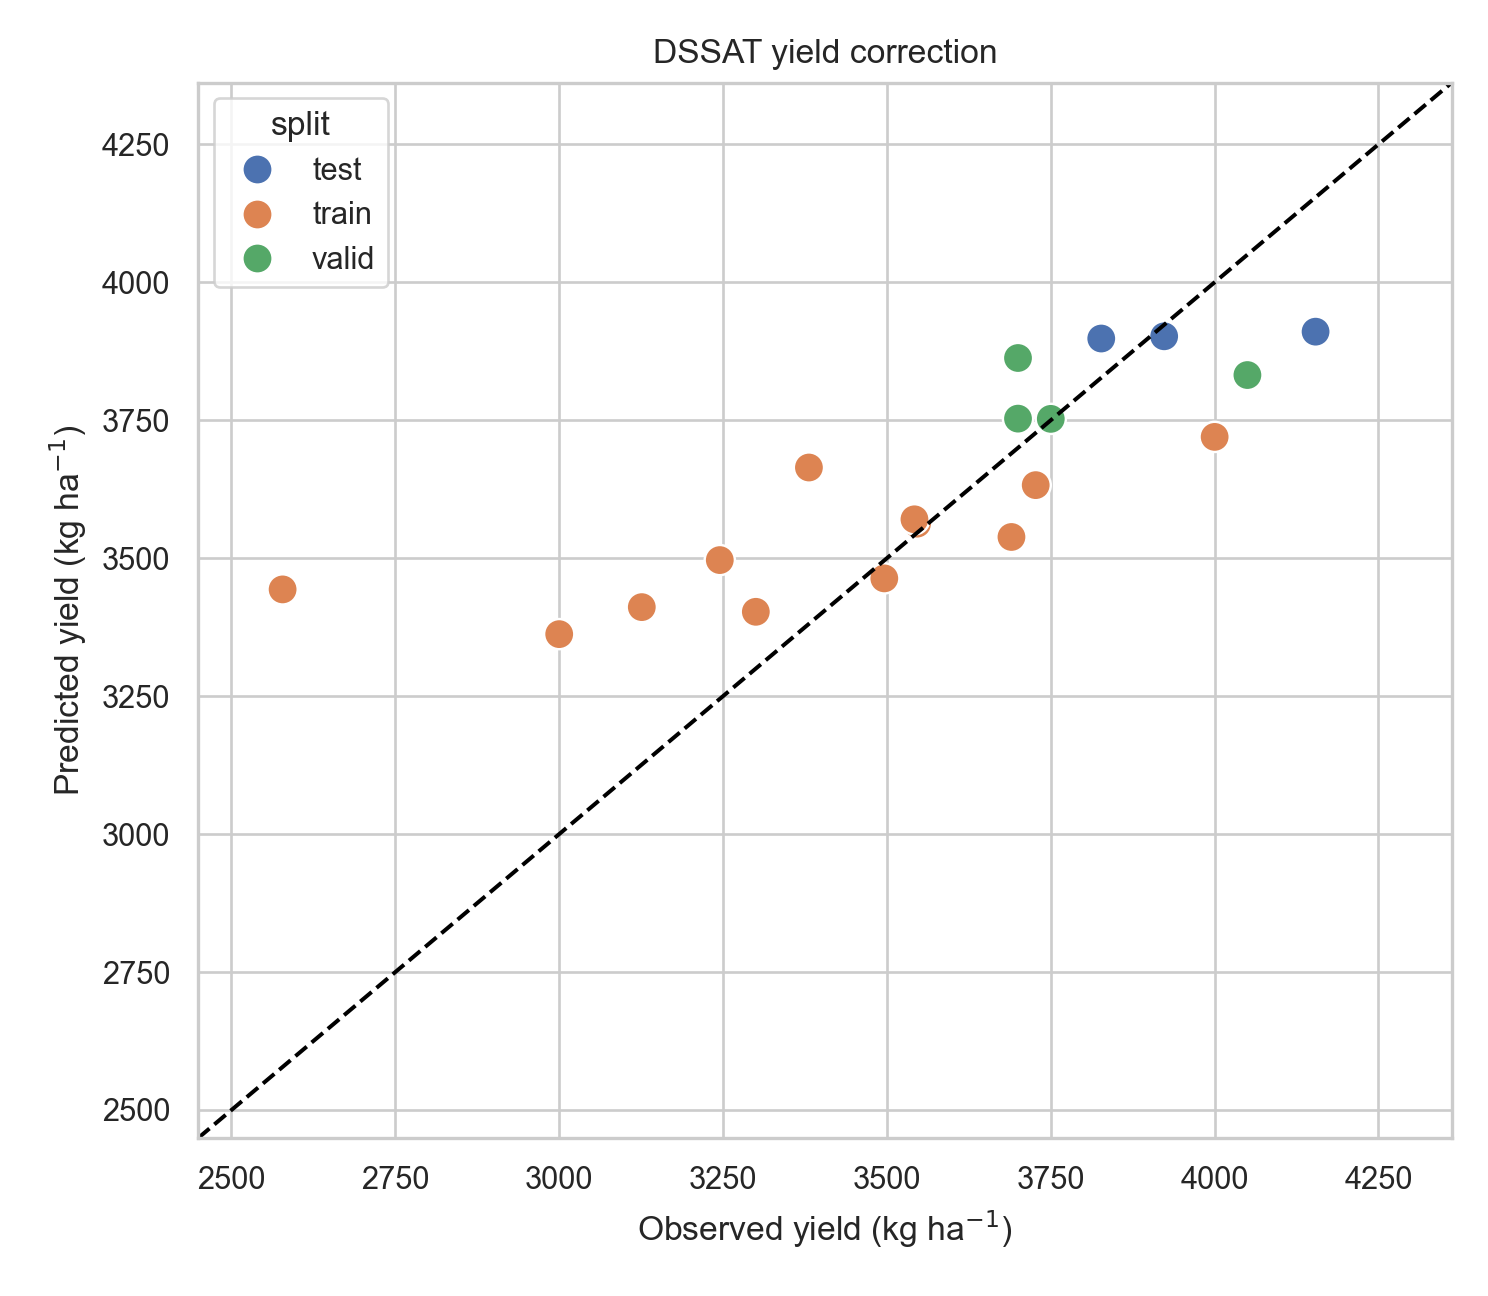
\includegraphics[scale=0.55]{fig_dssat_obs_pred.png}
\caption{Observed municipal yield and corrected yield in the previous diagnostic configuration. Each point represents one season and corresponds to the mean corrected yield over five sowing dates; the independent sample sizes are $n=12$, $n=4$, and $n=3$ for training, validation, and diagnostic sets, respectively. The figure documents the behaviour of the statistical correction and is not interpreted as crop-model validation.}
\label{fig:dssat_obs_pred}
\end{figure}

\begin{figure}[!h]
\centering
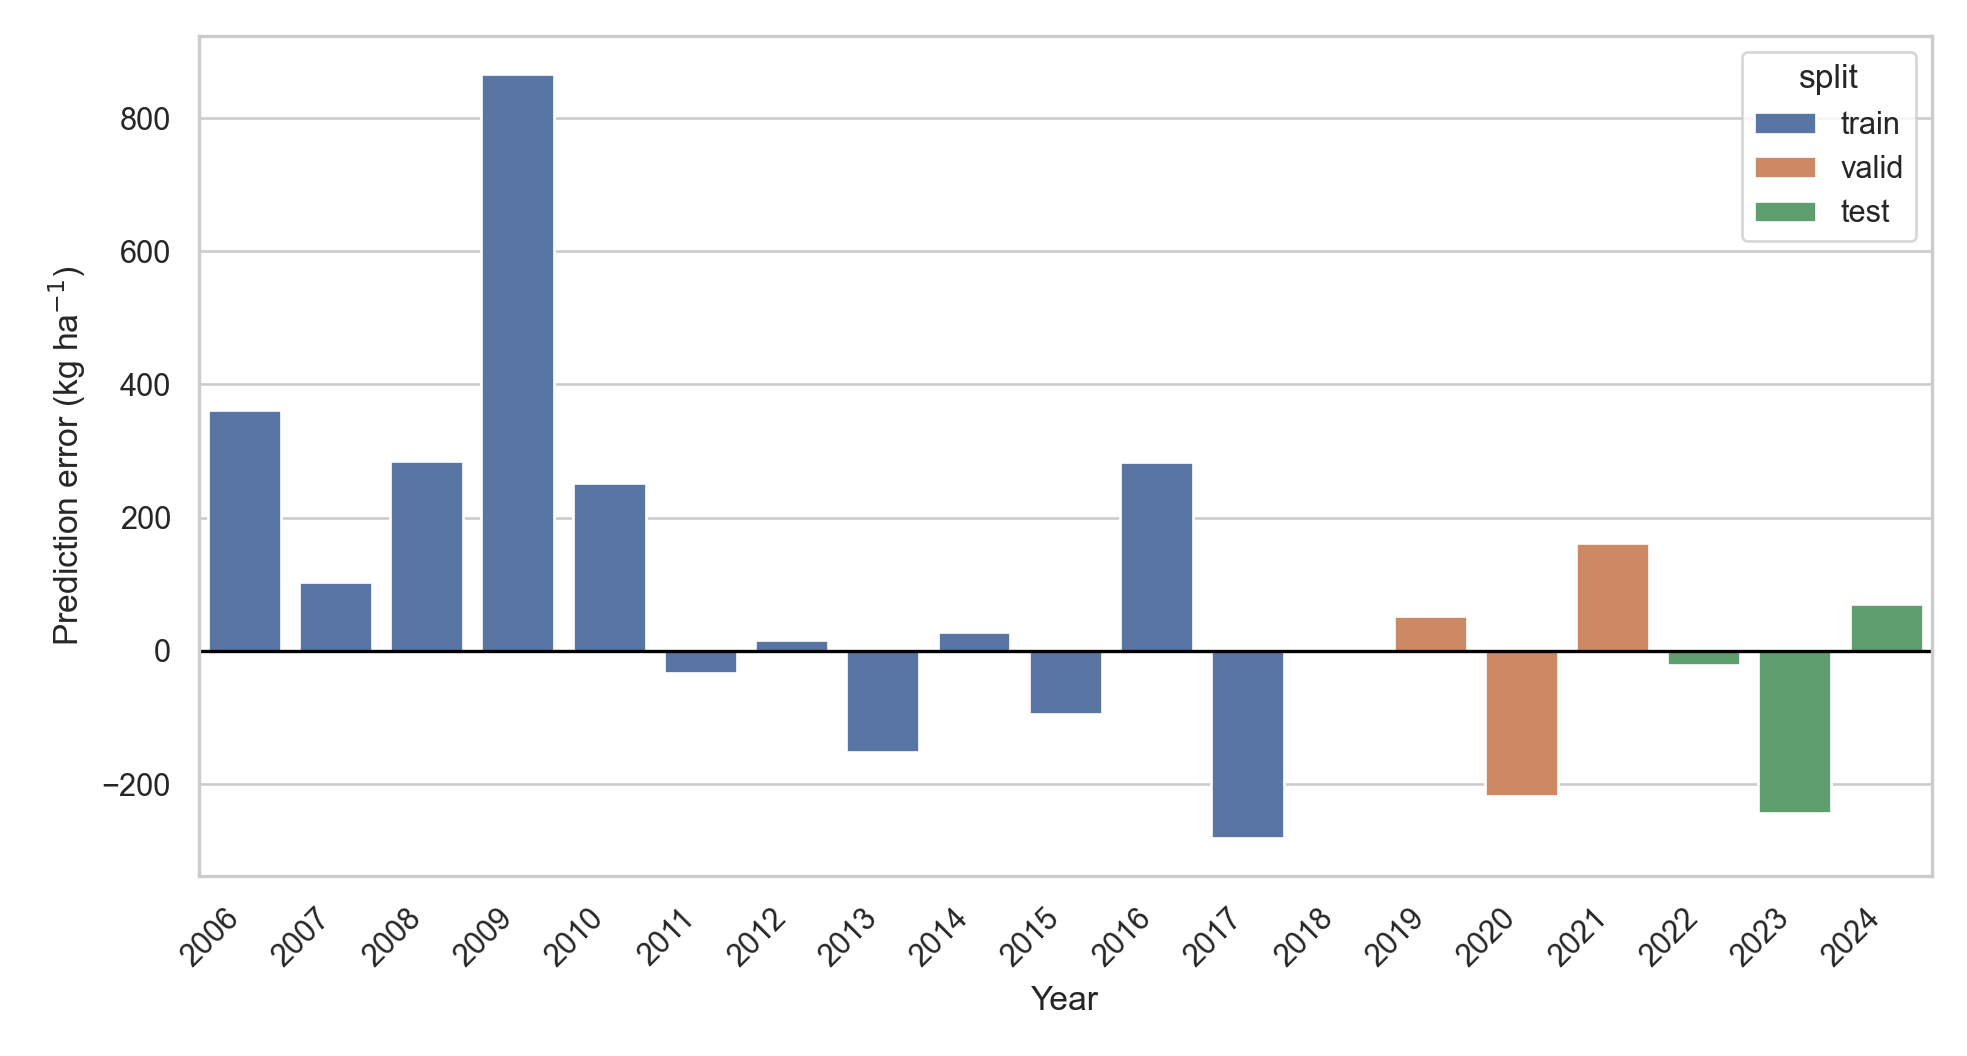
\includegraphics[scale=0.55]{fig_dssat_erro_ano.png}
\caption{Annual error of corrected yield relative to the municipal SIDRA series in the previous diagnostic configuration. The 2018 error is $+2.47$ kg ha$^{-1}$ and is shown numerically because the corresponding bar is below the plot resolution.}
\label{fig:dssat_erro_ano}
\end{figure}

Figures~\ref{fig:dssat_obs_pred} and~\ref{fig:dssat_erro_ano} document how the statistical transformation tracked the municipal series. They do not establish that the crop model reproduced field-scale yield responses to sowing date or irrigation. The final configuration therefore separates field-scale crop-model calibration and validation from municipal contextual verification and does not use agreement with SIDRA as a measure of policy performance.

%%============================================================
\subsubsection{Training trajectory and checkpoint behaviour}
\label{subres_diagnostic_training}

The optimization trajectory from the previous configuration is retained to document the behaviour of the original training procedure. It was produced with a single training seed and with an earlier statistical correction and optimization-function parameterization. The resulting training curve is therefore not directly comparable with the final evaluation configuration and is not reused for checkpoint selection in the final analysis.

\begin{table}[!h]
\centering
\caption{Selected points from the PPO validation trajectory in the previous configuration. Training used $\kappa = 0.0035$ mm$^{-1}$ and the statistical correction available at that stage. The reported SD is calculated over 64 resampled episodes derived from four validation seasons and therefore does not represent 64 independent environmental scenarios.}
\label{tab_curva_validacao}
\begin{tabular}{rrrrr}
\hline
Steps & Mean optimization function & SD & Mean corrected yield & Mean irrigation \\
      &                            &    & (kg ha$^{-1}$) & (mm) \\
\hline
10,000  & 0.669 & 0.433 & 3,661.91 & 58.02 \\
50,000  & 0.683 & 0.504 & 2,944.47 & 5.25  \\
90,000  & 0.699 & 0.504 & 3,019.88 & 5.69  \\
130,000 & 0.590 & 0.507 & 2,562.08 & 5.81  \\
170,000 & 0.648 & 0.529 & 2,798.09 & 5.09  \\
\hline
\end{tabular}
\end{table}

The highest recorded mean validation optimization function occurred at 90,000 steps, whereas training stopped at 170,000 steps after the predefined sequence of evaluations without improvement. However, the corrected-yield values produced during training differ from those obtained when the policy was subsequently evaluated with the later statistical correction. The trajectory therefore provides a diagnostic of the original optimization process rather than evidence of performance under the final frozen environment.

\begin{figure}[!h]
\centering
\begin{subfigure}[b]{0.49\linewidth}
\centering
\includegraphics[width=\linewidth]{validation_model_selection_en.png}
\caption{Mean validation optimization function, $\pm 1$ SD band, and selected checkpoint.}
\end{subfigure}
\hfill
\begin{subfigure}[b]{0.49\linewidth}
\centering
\includegraphics[width=\linewidth]{validation_yield_irrigation_en.png}
\caption{Mean corrected yield and mean irrigation during validation episodes.}
\end{subfigure}
\caption{Validation trajectory recorded during PPO training in the previous configuration. The trajectory was obtained with a single training seed and an environment definition that was subsequently modified; it is retained as a methodological diagnostic and is not used as evidence of training stability in the final configuration.}
\label{fig:validation_learning_curve}
\end{figure}

%%============================================================
\subsubsection{Policy outputs across development scenarios}
\label{subres_diagnostic_policy}

Re-evaluation of the policy from the previous configuration showed limited variation in the selected management action across the available seasonal contexts. Sowing dates remained between late September and early October, while the irrigation trigger and irrigation depth remained at the boundaries of the original action space. Seasonal irrigation was zero in nearly all evaluated seasons. These results are retained because the action-bound behaviour contributed directly to the redesign of the final action space and to the explicit inclusion of a rainfed option. They are not interpreted as evidence that the final contextual policy converges to the same management strategy.

\begin{table}[!h]
\centering
\scriptsize
\caption{Per-scenario results of the policy from the previous diagnostic configuration. The evaluation used a single training seed and corrected yield. Observed municipal yield is shown only for contextual comparison. The irrigation trigger was $\theta=90$ mm and irrigation depth was $l=2$ mm in all scenarios, corresponding to action-space boundaries. The 2025 season is an unobserved simulation scenario and is not part of the empirical 2022--2024 diagnostic set.}
\label{tab_ppo_scenarios}
\begin{tabular}{llrrrrrrrr}
\hline
Set & Season & Sowing date & $L$ (mm) & Irrigation (mm) & Rainfall (mm) & Corrected yield (kg ha$^{-1}$) & Observed (kg ha$^{-1}$) & Error (kg ha$^{-1}$) & $r$ \\
\hline
Validation & 2018 & 29/09 & 32.99 & 0 & 738 & 3,763.59 & 3,750 & 13.59   & 0.896 \\
Validation & 2019 & 02/10 & 30.74 & 0 & 573 & 3,773.91 & 3,700 & 73.91   & 0.899 \\
Validation & 2020 & 30/09 & 32.14 & 0 & 667 & 3,830.71 & 4,050 & -219.29 & 0.912 \\
Validation & 2021 & 27/09 & 36.44 & 0 & 641 & 3,864.08 & 3,700 & 164.08  & 0.920 \\
Diagnostic & 2022 & 27/09 & 35.95 & 0 & 714 & 3,904.62 & 3,923 & -18.38  & 0.930 \\
Diagnostic & 2023 & 29/09 & 32.95 & 0 & 844 & 3,943.61 & 4,154 & -210.39 & 0.939 \\
Diagnostic & 2024 & 02/10 & 29.40 & 2 & 647 & 3,936.53 & 3,827 & 109.53  & 0.934 \\
Unobserved scenario & 2025 & 27/09 & 36.26 & 0 & 623 & 4,017.29 & -- & -- & 0.956 \\
\hline
\end{tabular}
\end{table}

Table~\ref{tab_ppo_scenarios} shows that $\theta$ remained at its upper bound and $l$ at its lower bound in every reported scenario. Irrigation was zero in all seasons except 2024, when 2 mm was applied. The limited variation in management actions indicates that the previous configuration did not provide evidence of a materially context-dependent policy. Because the state contained retrospective seasonal information and the statistical correction dominated the management response, this behaviour cannot be attributed to crop physiology or to an operational value of pre-season information.

%%============================================================
\subsubsection{Comparison with constructed reference schedules}
\label{subres_diagnostic_schedules}

The previous policy was also compared descriptively with four constructed reference schedules. These comparisons were performed before the inclusion of an optimized fixed rule, a context-free optimizer, and a simple contextual comparator. They therefore quantify only the difference between the previous policy and the constructed schedules and do not isolate the value of contextual adaptation or the incremental value of PPO.

\begin{table}[!h]
\centering
\footnotesize
\caption{Optimization function, corrected yield, and irrigation for the policy from the previous diagnostic configuration and the constructed reference schedules. The evaluation used a single training seed and $\kappa=0.0015$ mm$^{-1}$. The 2022--2024 seasons constitute the empirical diagnostic set; the 2025 unobserved simulation scenario is included only in the descriptive four-season mean shown in the right-hand block and is not treated as an independent empirical validation season. These means are not used as the primary comparative result of the final study.}
\label{tab_comparacao_baselines}
\begin{tabular}{lrrrrrr}
\hline
 & \multicolumn{3}{c}{Validation (2018--2021)} & \multicolumn{3}{c}{Diagnostic/development scenarios (2022--2025)$^{a}$} \\
Policy & $r$ & Yield (kg ha$^{-1}$) & Irrig.\ (mm) & $r$ & Yield (kg ha$^{-1}$) & Irrig.\ (mm) \\
\hline
PPO (previous configuration) & 0.907 & 3,808.07 & 0.00 & 0.940 & 3,950.51 & 0.50 \\
Rainfed Oct/15              & 0.906 & 3,805.81 & 0.00 & 0.939 & 3,945.76 & 0.00 \\
Irrigated Sep/25            & 0.871 & 3,800.02 & 22.50 & 0.919 & 3,944.88 & 13.50 \\
Irrigated Oct/15            & 0.864 & 3,796.99 & 27.00 & 0.881 & 3,926.69 & 36.00 \\
Irrigated Nov/10            & 0.871 & 3,801.42 & 22.50 & 0.861 & 3,926.78 & 49.50 \\
\hline
\multicolumn{7}{l}{\scriptsize $^{a}$The 2025 season is an unobserved simulation scenario and is included only in this descriptive mean.}
\end{tabular}
\end{table}

The estimated differences between the previous policy and the rainfed October 15 schedule were numerically small in both temporal blocks, whereas the irrigated constructed schedules attained similar corrected yields with greater irrigation use. Such comparisons cannot establish the value of contextual adaptation because the statistical correction penalized irrigation independently of the explicit water penalty and because no optimized fixed rule, context-free optimizer, or simple contextual baseline was available. The final comparative analysis therefore replaces means of this type with paired differences in agronomic units, uncertainty across independent environment--season units, and explicit separation of environmental and algorithmic variability.

Taken together, the diagnostic evidence identifies four properties that prevent the previous configuration from supporting the final agronomic interpretation: the crop model had not yet been calibrated at field scale; the statistical transformation dominated the corrected management response; the policy received retrospective seasonal information unavailable at the decision time; and the optimization was represented by a single training seed without the final comparator structure or an untouched external test. The diagnostic results are therefore retained as evidence motivating the methodological redesign, whereas all conclusions regarding crop-model validity, contextual adaptation, productivity--water performance, risk, and external generalization are reserved for the final frozen experimental configuration.

%%============================================================
\subsection{Crop-model validity and data quality}
\label{subres_validity}

\textcolor{red}{\textbf{FAZER:} Validar agronomicamente o DSSAT com dados de campo ou ensaio: fenologia observada $\times$ simulada, produtividade observada $\times$ simulada, erro por ambiente, água no solo quando disponível, partições separadas de calibração e validação, e sem misturar SIDRA municipal com ensaio de campo.}

The computational audit added after review generated the weather-completeness table by season and the season--SIDRA pairing table. These files are stored as \texttt{weather\_completeness\_by\_season.csv} and \texttt{season\_sidra\_pairing\_audit.csv}. The corrected weather summary removed the previous artefact in \texttt{weather\_splits.md}; mean seasonal temperatures are now within the observed range of the station. In the seasons used by the current diagnostic split, invalid precipitation days were concentrated in 2014--2016 and 2022--2025, confirming that imputation strategy can affect exactly the dry seasons used for management interpretation. The SIDRA audit records both candidate pairings: sowing year $y$ and harvest year $y+1$. This table does not resolve the official PAM convention, but it makes the boundary-year choice explicit and reproducible.

\begin{table}[!h]
\centering
\scriptsize
\caption{Selected weather-completeness diagnostics generated from the consolidated hourly series. Values are seasonal aggregates from September of year $y$ to April of year $y+1$.}
\label{tab_weather_completeness_diag}
\begin{tabular}{lrrrrr}
\hline
Split & Seasons & Rain invalid days & Temp. invalid days & Mean rainfall & Mean temp. \\
      &         & (mean) & (mean) & (mm) & ($^\circ$C) \\
\hline
Training & 2006--2017 & 51.1 & 14.1 & 1299.6 & 17.4 \\
Validation & 2018--2021 & 57.3 & 0.0 & 1044.2 & 17.2 \\
Diagnostic & 2022--2025 & 102.0 & 12.8 & 979.8 & 18.7 \\
\hline
\end{tabular}
\end{table}

\emph{Current run (development environment).} With the generic configuration, the raw DSSAT yield ranged from 1,918 to 5,925 kg ha$^{-1}$ across sowing dates and seasons, its annual absolute deviation from the municipal series was 208--2,300 kg ha$^{-1}$ and its correlation with that series 0.04 over 95 rows (19 seasons $\times$ 5 sowing dates). The statistical correction was fitted on 60 rows (12 training seasons $\times$ 5 dates) with $\alpha = 200$ selected among $\{0.05,\dots,500\}$ and an intercept adjustment of $+136.40$ kg ha$^{-1}$ (fitted coefficients in Supplementary Table S4, $Y_{\text{ref}} = 4200$ kg ha$^{-1}$ in the outcome). Its fitted coefficient for the raw yield was $-0.0065$, the correlation between raw and corrected yield was 0.07, within a season the five sowing dates spanned up to 1,578 kg ha$^{-1}$ of raw yield but only 2--48 kg ha$^{-1}$ of corrected yield, and its irrigation coefficients were negative ($-0.106$ per mm, rain--irrigation interaction $-0.361$), so irrigation lowered the corrected yield independently of $\kappa$. The correction reproduced the municipal series with MAE of 229.56, 109.06, and 111.82 kg ha$^{-1}$ in training, validation, and the 2022--2024 diagnostic seasons (validation bias zero by construction), by compressing the interannual variance toward the trend, the largest training deviation was 2009 (+865 kg ha$^{-1}$) and the 2018 error was +2.47 kg ha$^{-1}$ (Appendix Tables~\ref{tab_metricas_calibracao}--\ref{tab_calibracao_ano}, Figs.~\ref{fig:dssat_obs_pred}--\ref{fig:dssat_erro_ano}). These figures describe the correction, not the crop model, a low MAPE here is not evidence of crop-model quality. \textcolor{red}{\textbf{FAZER:} Tabela de ablação no Suplemento S4, feita em desenvolvimento, e a decisão sobre a correção, registrada aqui.}

%%============================================================ 
\subsection{Training stability and out-of-sample paired effects}
\label{subres_performance}

\textcolor{red}{\textbf{FAZER:} Executar a rodada final com pelo menos cinco sementes, preferencialmente dez, usando o contexto operacional em $t_0$, comparadores finais e teste externo fechado.}

\emph{Current run (development environment).} Training with a single seed (42) and $\kappa = 0.0035$ mm$^{-1}$ reached its best validation outcome (0.699) at 90,000 steps and stopped at 170,000 after eight evaluations without improvement, the mean corrected yields of the validation seasons during training (2,277--3,662 kg ha$^{-1}$) lie outside the range produced by the final correction for the same seasons (3,746--3,864 kg ha$^{-1}$), because an earlier correction was in use, so the training curve is not comparable with the evaluation and the checkpoint is not reused (Appendix Table~\ref{tab_curva_validacao}, Fig.~\ref{fig:validation_learning_curve}). Re-evaluated with the final correction and $\kappa = 0.0015$ mm$^{-1}$, the policy sowed between September 27 and October 2 in all eight validation and diagnostic seasons, with $\theta = 90$ mm and $l = 2$ mm --- the upper bound of $\theta$ and the lower bound of $l$ --- and a cap of 29--36 mm never reached, irrigation was 0 mm in seven seasons and 2 mm in 2024. Mean corrected yield was 3,808 kg ha$^{-1}$ (validation) and 3,951 kg ha$^{-1}$ (diagnostic set), the decision did not change across contexts beyond a five-day shift of the sowing date (Appendix Table~\ref{tab_ppo_scenarios}). The agreement of the corrected yields with the municipal series (MAE 112.77 kg ha$^{-1}$) equals that of the correction itself and is not a measure of the policy.

The seed-level diagnostic files now report the single available seed explicitly instead of implying replication. Seed 42 produced mean rewards of 0.907 in validation and 0.940 in the diagnostic set, with no failed DSSAT runs. Action-bound diagnostics showed that the irrigation trigger was at its upper bound in 100\% of validation and diagnostic scenarios, the event depth was at the lower bound in 100\%, and realized rainfed management occurred in 100\% of validation seasons and 75\% of diagnostic seasons. Therefore, under the previous configuration, the learned policy behaved mostly as a near-fixed late-September calendar with little irrigation.

\begin{table}[!h]
\centering
\scriptsize
\caption{Seed and action-bound diagnostics for the current development run.}
\label{tab_seed_action_diag}
\begin{tabular}{lrrrrrr}
\hline
Split & Seed & Scenarios & Reward & Yield & Irrigation & Rainfed freq. \\
      &      &           & mean   & (kg ha$^{-1}$) & (mm) & \\
\hline
Validation & 42 & 4 & 0.907 & 3808.1 & 0.0 & 1.00 \\
Diagnostic & 42 & 4 & 0.940 & 3950.5 & 0.5 & 0.75 \\
\hline
\end{tabular}
\end{table}

\begin{figure}[!h]
\centering
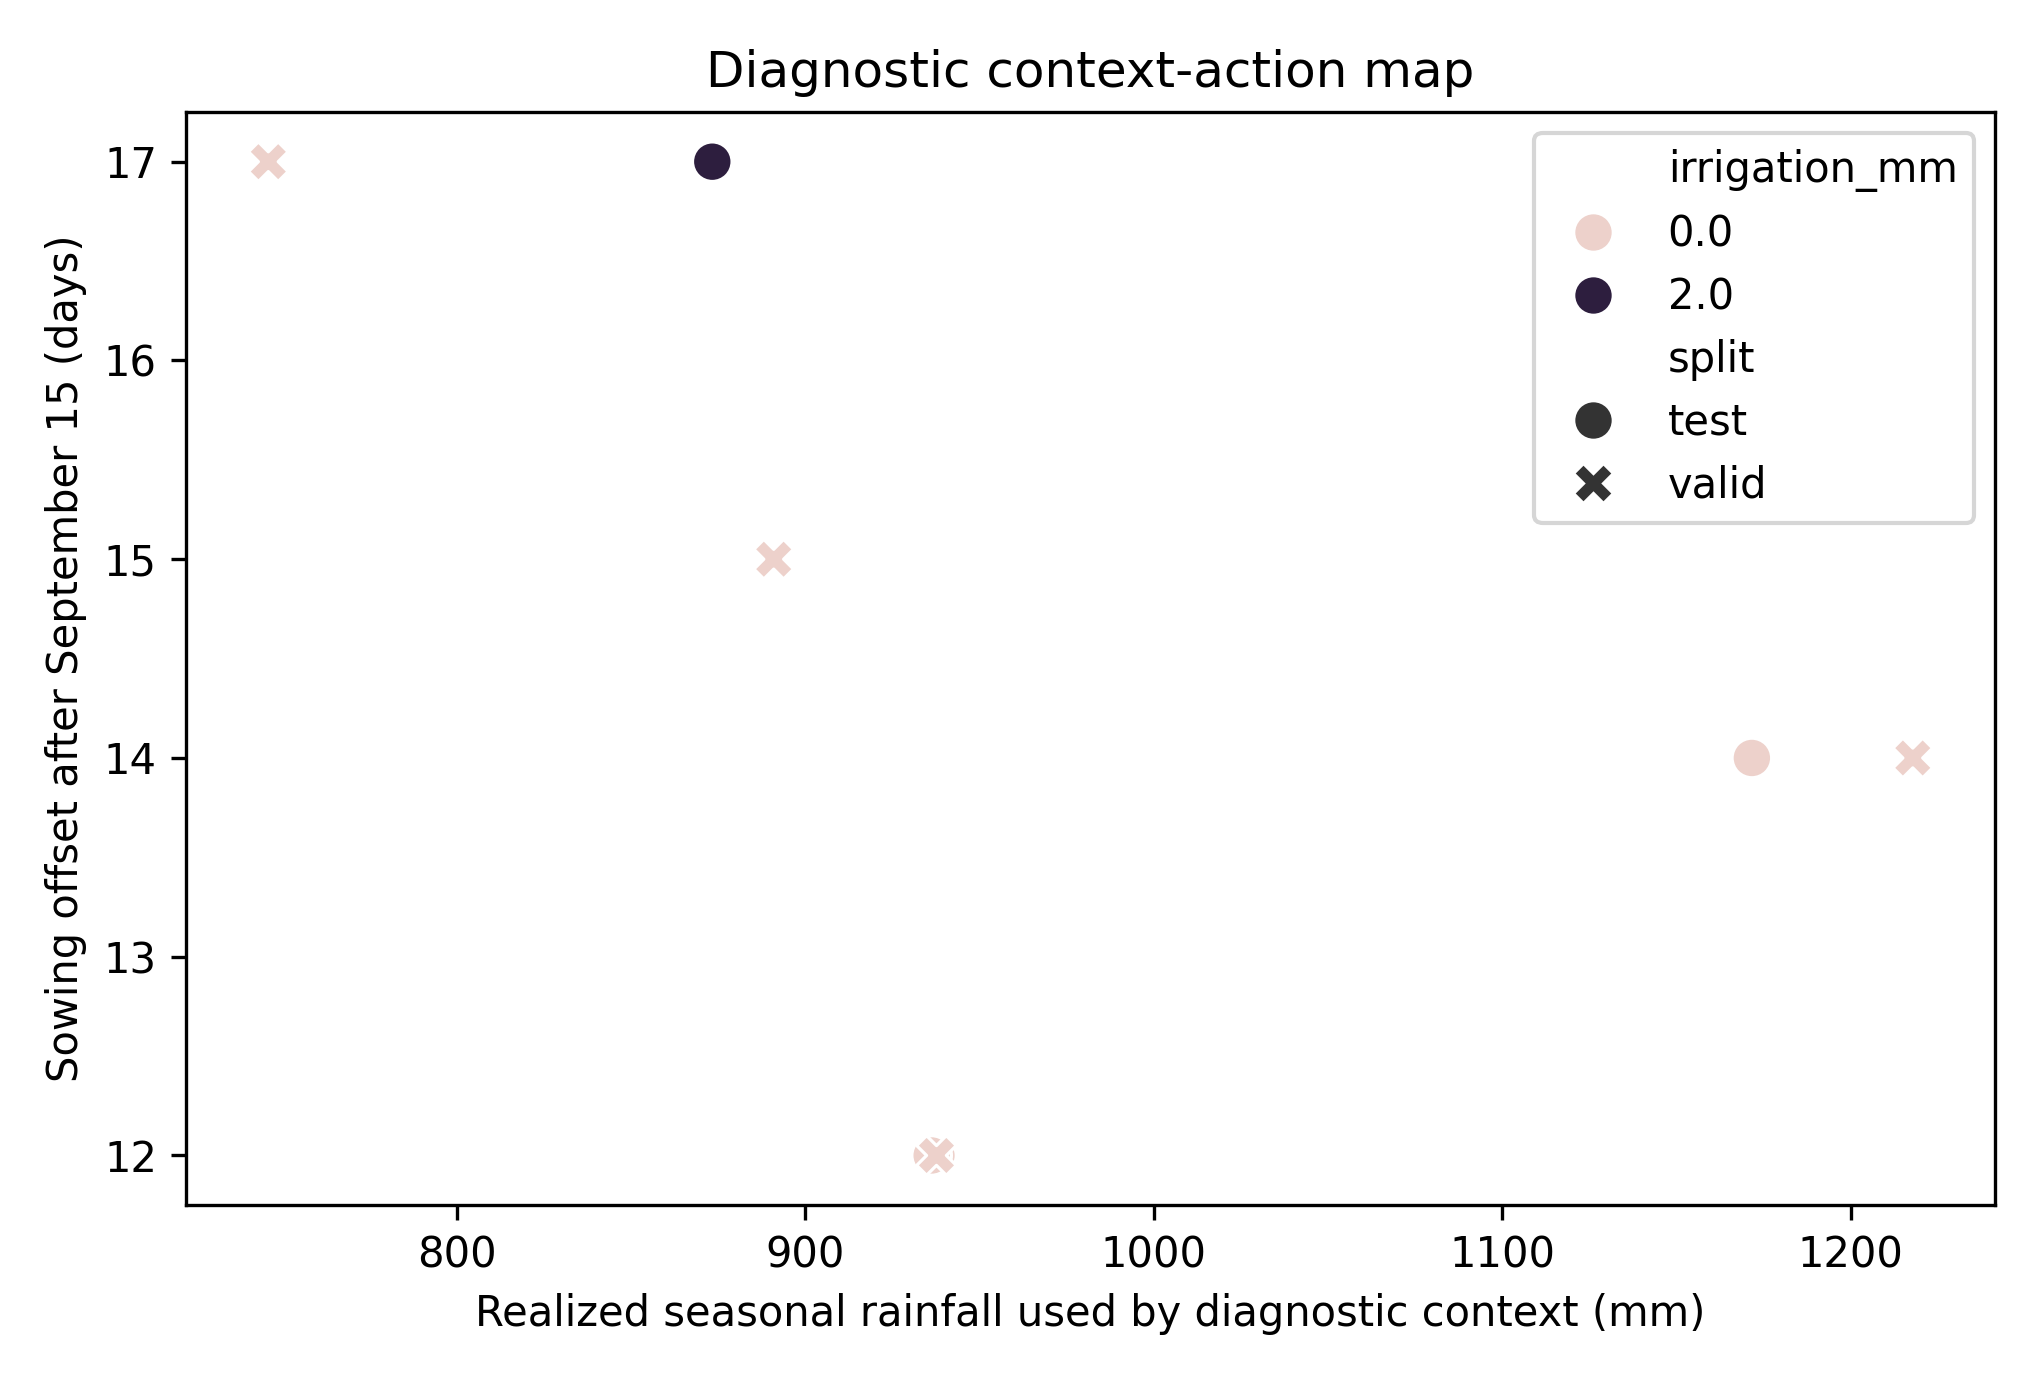
\includegraphics[width=0.75\linewidth]{dssat_rl_soybean/outputs/ppo_soja_castro_dssat/figures/diagnostic_context_action_map_en.png}
\caption{Diagnostic context--action map from the previous configuration. The horizontal axis uses realized seasonal rainfall and is therefore not an operational context available at $t_0$.}
\label{fig_context_action_diag}
\end{figure}

%%============================================================ 
\subsection{Value of adaptation versus fixed, contextual, and optimization baselines}

\label{subres_value}

\textcolor{red}{\textbf{FAZER:} Executar os três contrastes primários finais: PPO contra regra fixa otimizada, baseline contextual simples e melhor otimizador livre de contexto, todos com o mesmo orçamento de chamadas DSSAT.}

\emph{Current run (development environment, diagnostic only).} Against the four constructed reference schedules, the corrected yield of the policy exceeded that of the rainfed October 15 schedule by 2.3 kg ha$^{-1}$ in validation and 4.8 kg ha$^{-1}$ in the diagnostic seasons, with irrigation of 0.0 and 0.5 mm against 0.0 mm, these differences are unresolved under the available independent seasons (four per set, one seed). The irrigated schedules produced similar corrected yields (3,797--3,801 and 3,927--3,945 kg ha$^{-1}$) with 13.5--49.5 mm of irrigation, their lower optimization function (0.861--0.919 vs 0.940) reflects the water penalty applied both by $\kappa$ and by the correction (Appendix Table~\ref{tab_comparacao_baselines}). No optimized fixed rule, context-free optimizer, or simple contextual baseline was run, so the value of adaptation cannot be assessed from the current run, and these numbers are not used to answer the four questions.

The paired diagnostic table now reports each constructed comparison by season. In the diagnostic seasons, PPO exceeded the rainfed October 15 schedule by 4.8 kg ha$^{-1}$ on average and used 0.5 mm more water. Against the irrigated constructed schedules, the mean paired yield difference ranged from 5.6 to 23.8 kg ha$^{-1}$, while PPO used 13.0--49.0 mm less irrigation. These are descriptive paired differences for constructed schedules only; they do not isolate the value of contextual adaptation.

\begin{table}[!h]
\centering
\scriptsize
\caption{Paired diagnostic differences between PPO and constructed schedules. Positive yield values favor PPO.}
\label{tab_paired_constructed_diag}
\begin{tabular}{llrrrr}
\hline
Split & Comparator & Seasons & Seeds & $\Delta$ yield & $\Delta$ irrigation \\
      &            &         &       & (kg ha$^{-1}$) & (mm) \\
\hline
Validation & Rainfed Oct 15 & 4 & 1 & 2.3 & 0.0 \\
Validation & Early Sep 25 irrigated & 4 & 1 & 8.1 & -22.5 \\
Diagnostic & Rainfed Oct 15 & 4 & 1 & 4.8 & 0.5 \\
Diagnostic & Early Sep 25 irrigated & 4 & 1 & 5.6 & -13.0 \\
Diagnostic & Oct 15 irrigated & 4 & 1 & 23.8 & -35.5 \\
Diagnostic & Nov 10 irrigated & 4 & 1 & 23.7 & -49.0 \\
\hline
\end{tabular}
\end{table}

\begin{figure}[!h]
\centering
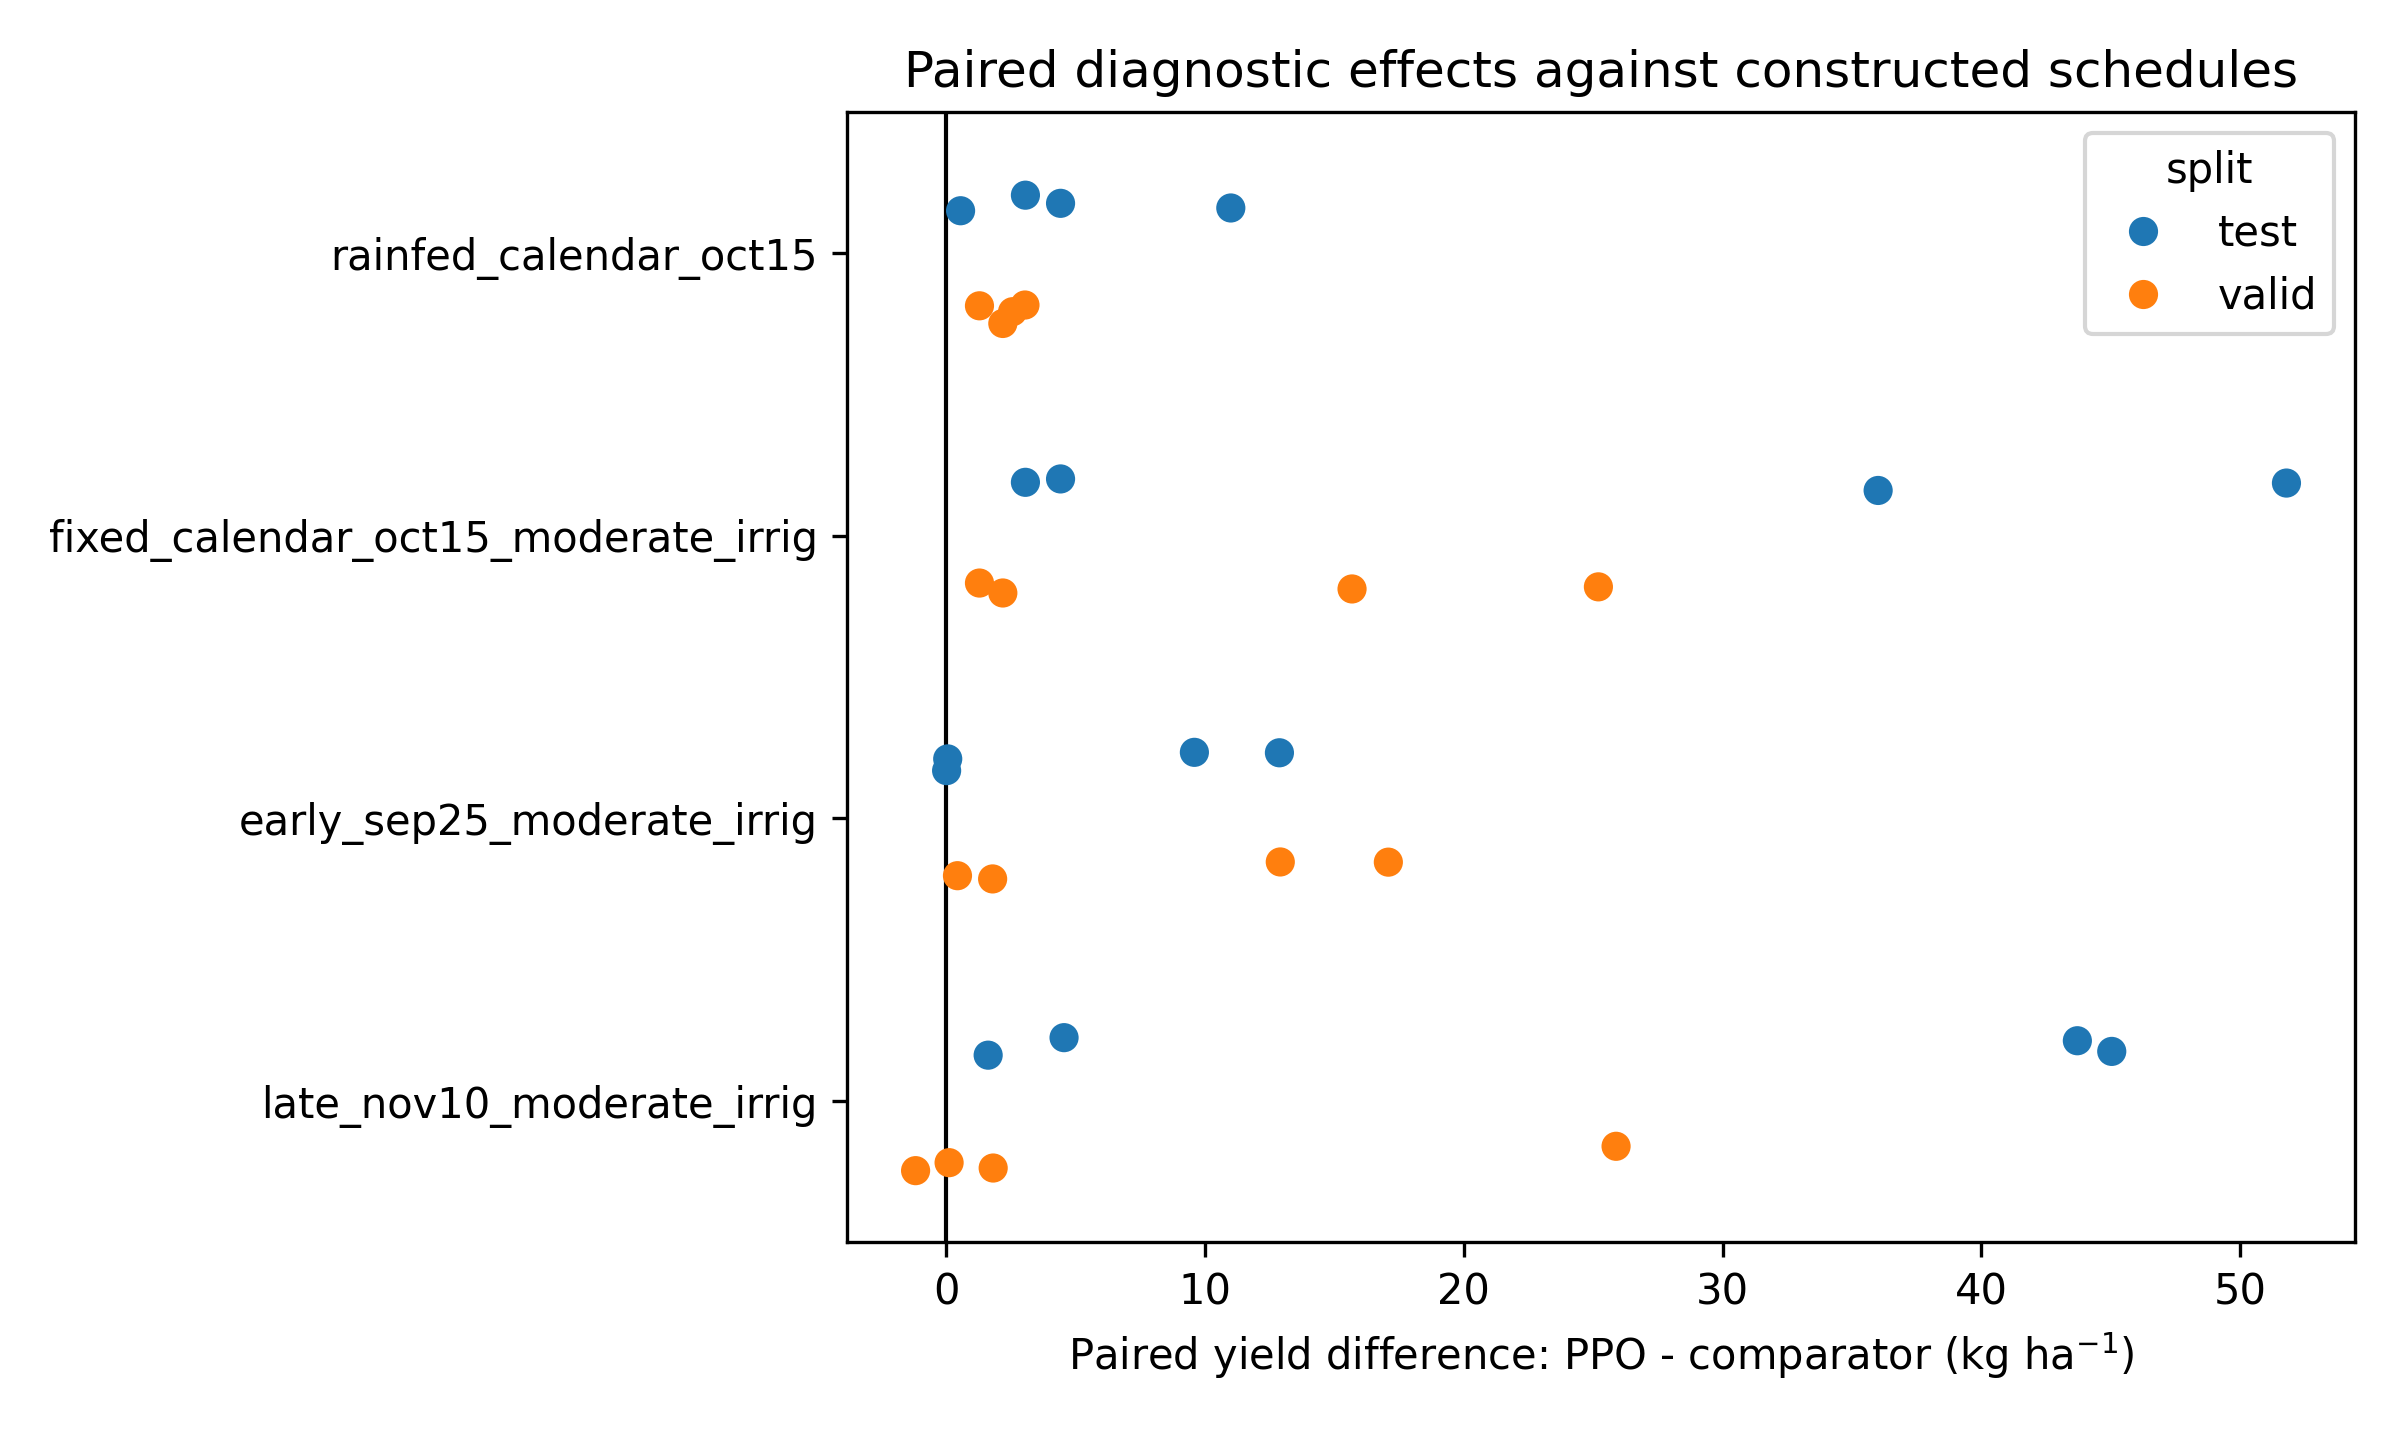
\includegraphics[width=0.78\linewidth]{dssat_rl_soybean/outputs/ppo_soja_castro_dssat/figures/paired_effects_vs_constructed_schedules_en.png}
\caption{Paired diagnostic yield differences between PPO and constructed schedules. Points are season-level paired differences; the comparison is diagnostic because optimized fixed and contextual baselines were not yet executed.}
\label{fig_paired_constructed_diag}
\end{figure}

%%============================================================ 
\subsection{Productivity--water frontier and risk}
\label{subres_tradeoff}

\textcolor{red}{\textbf{FAZER:} Retreinar a fronteira produtividade--água final com pelo menos cinco valores de $\kappa$ ou custo de água, usando o contexto operacional e sem escolher pontos com base no teste externo.}

For the diagnostic run, risk was summarized with the 10th percentile of yield and CVaR$_{10}$ across the available scenarios. In the diagnostic seasons, PPO had mean yield of 3950.5 kg ha$^{-1}$, mean irrigation of 0.5 mm, 10th percentile yield of 3914.2 kg ha$^{-1}$, and CVaR$_{10}$ of 3904.6 kg ha$^{-1}$. The rainfed October 15 schedule had mean yield of 3945.8 kg ha$^{-1}$, 0.0 mm irrigation, 10th percentile yield of 3910.9 kg ha$^{-1}$, and CVaR$_{10}$ of 3901.6 kg ha$^{-1}$. These differences are small and remain descriptive because the run used one seed and constructed schedules.

\begin{figure}[!h]
\centering
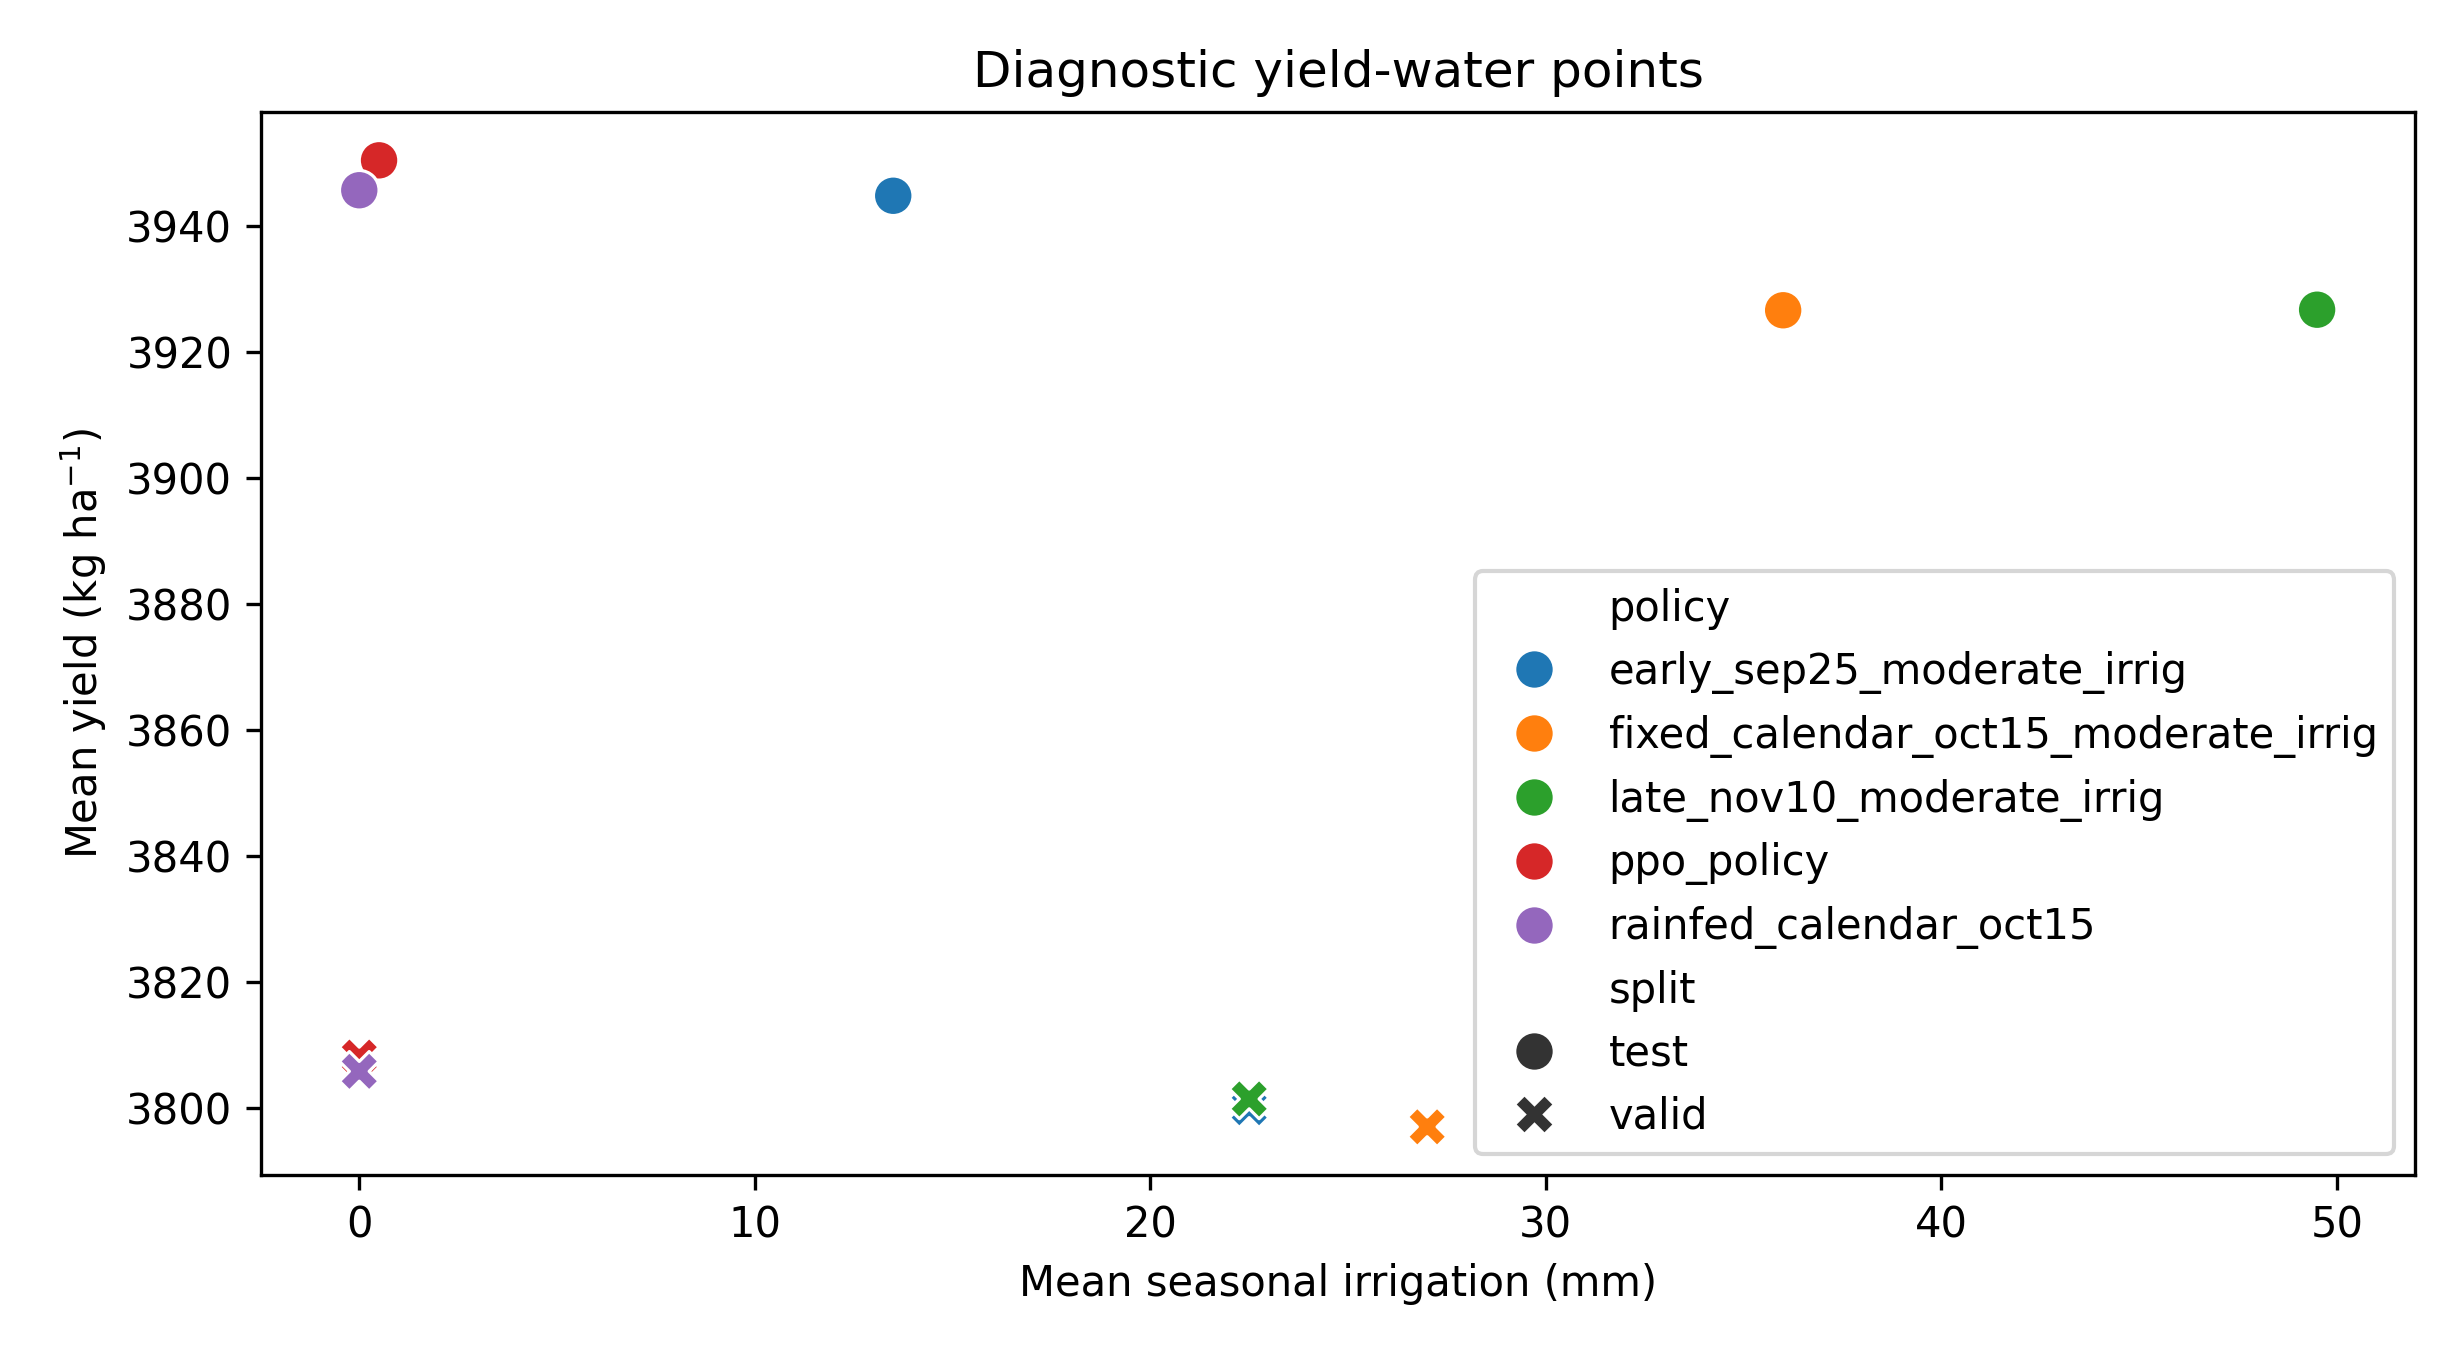
\includegraphics[width=0.78\linewidth]{dssat_rl_soybean/outputs/ppo_soja_castro_dssat/figures/diagnostic_yield_water_points_en.png}
\caption{Diagnostic yield--water points for PPO and constructed schedules. This is not the final Pareto frontier because policies were not retrained over multiple water-cost settings.}
\label{fig_yield_water_diag}
\end{figure}

%%============================================================ 
\subsection{Robustness and external generalization}
\label{subres_generalization}

\textcolor{red}{\textbf{FAZER:} Executar generalização externa com mais ambientes, \emph{leave-one-location-out}, análise de valor da informação e sensibilidade a imputação, \emph{spin-up}, limites da ação e parâmetros calibrados do modelo de cultivo.}

The current study still contains one environment only. Generalization among environments was therefore not tested. The action-bound audit showed 100\% saturation at the upper irrigation trigger and 100\% saturation at the lower event depth in both validation and diagnostic sets. This supports the interpretation that the previous policy did not express a context-dependent irrigation strategy. The software now records these frequencies in \texttt{action\_bound\_saturation.csv}, but the agronomic explanation requires the final run with a calibrated crop model and valid $t_0$ context.

% =====================================================================
\section{Discussion}
\label{discussao}


\textcolor{red}{\textbf{FAZER:} A partir da evidência final, não pelo preenchimento dos marcadores: organizar em torno de quatro perguntas --- por que o contexto alterou ou não a decisão, em quais ambientes, qual a magnitude da vantagem ou perda, sob quais restrições de água a adaptação apresentou ou não valor ---, relacionando chuva antecedente, armazenamento de água no solo, fenologia, data de semeadura, disponibilidade hídrica e comportamento da política, separar ganho por boa regra fixa, ganho por adaptação e ganho adicional do algoritmo, tratar ausência de vantagem adaptativa como resultado válido, sem convertê-la em superioridade metodológica.}

%%============================================================ 
\subsection{Mechanisms: climate--soil--sowing--water interaction}
\label{subdisc_mechanisms}

\textcolor{red}{\textbf{FAZER:} Após os Gates G0--G2 e A1--A7: como chuva antecedente e água inicial alteram o valor da data de semeadura, como a disponibilidade hídrica modifica o benefício da irrigação, quais contextos produzem mudança de decisão, quais safras/ambientes funcionam como casos contrastantes, se a política reage ao clima ou converge para uma data quase fixa, relacionar com a fenologia simulada. Figura E (contexto $\rightarrow$ ação) apenas com estados válidos em $t_0$.}

\emph{Current run.} No mechanism could be isolated: the corrected yield varied by only a few tens of kg ha$^{-1}$ across the whole sowing window and responded negatively to any applied water, because the statistical correction --- fitted to a municipal series in which management did not vary --- assigned the within-season response of the crop model to noise. The convergence of the policy to late-September sowing without irrigation is compatible with the objective and with the correction and cannot be attributed to crop physiology.

%%============================================================ 
\subsection{Value of context and information}
\label{subdisc_information}

\textcolor{red}{\textbf{FAZER:} Após C1 e A1: ganho incremental de regra fixa $\rightarrow$ climatologia $\rightarrow$ informação pré-safra $\rightarrow$ previsão histórica $\rightarrow$ oráculo retrospectivo (teto, não política operacional), robustez a erro de previsão (C4). Na rodada atual, o contexto continha o clima realizado da safra --- o que corresponde ao oráculo, não a uma situação operacional --- e mesmo assim a política não se distinguiu de um calendário fixo, a observação sugere que, neste sistema e sob esta correção, a informação perfeita não alterou a decisão, o que deve ser testado com o simulador validado.}

%%============================================================ 
\subsection{When an adaptive policy is worth the complexity}
\label{subdisc_value}

In the current run the difference in corrected yield between the policy and rainfed sowing on October 15 was a few kg ha$^{-1}$ and unresolved (Section~\ref{subres_value}), this is consistent with \citet{kelly2024assessing}, in whose AquaCrop-OSPy experiments deep RL irrigation policies did not outperform an optimized soil-moisture heuristic under high rainfall variability and paid off only under water scarcity or severe restrictions. The present design differs from that study and from \citet{balderas2025comparative} in the frequency of decision (once before the season, versus within-season actions on the simulated soil-water and nitrogen states), which bounds the value of adaptation that can be observed, and in the number of independent contexts. \textcolor{red}{\textbf{FAZER:} Após A5/A8/C2/C5: onde a política agrega ou não agrega valor sobre a regra fixa otimizada, a baseline contextual simples e o otimizador livre de contexto, magnitude do efeito e incerteza, custo computacional por método contado em todas as chamadas, decomposição boa regra fixa + adaptação + algoritmo. Comparar com Kelly, Balderas e Noa-Yarasca somente nos eixos verificados nos artigos originais (frequência de decisão, informação disponível, dimensão da ação, número de cenários independentes, baseline, resultado central, contexto hídrico e grau de generalização), a tabela comparativa foi transferida ao Suplemento S6 até a verificação integral das células marcadas com *, e só retorna ao corpo se todas forem confirmadas.}

\textcolor{red}{\textbf{FAZER:} Retorna ao corpo somente após verificação, nos artigos originais, de frequência de decisão, informação fornecida ao agente, número de contextos e generalização de cada estudo.}

%%============================================================ 
\subsection{Resource allocation and risk}
\label{subdisc_resources}

\textcolor{red}{\textbf{FAZER:} Após A4/B4/C3: fronteira água--produtividade ou água--margem, custo ou peso da água a partir do qual a irrigação suplementar entra na política, desempenho nos anos adversos (percentil 10, CVaR, \emph{regret}), implicações para a alocação de água e para as restrições reais de operação em nível de fazenda. Qualquer afirmação operacional depende de: contexto formado com informação disponível em $t_0$, validação externa, modelo de cultivo calibrado, cenário realista de custo ou limite de água, análise de incerteza. Na rodada atual a irrigação foi penalizada duas vezes e a análise não é interpretável, o método é, por ora, um potencial metodológico, não um suporte à decisão.}

%%============================================================ 
\subsection{Generalization and limitations}
\label{subdisc_limitations}

\textcolor{red}{\textbf{FAZER:} Após B1/B5/A10/A6: variabilidade entre sementes como estabilidade do algoritmo, entre ambientes como validade externa, impacto da imputação, do \emph{spin-up}, da saturação dos limites, LOLO, cenários em que a adaptação perde valor --- explicando qual componente do sistema controla a perda ou o ganho de robustez. Enquanto o estudo permanecer em uma localidade, declarar que a generalização não foi testada.}

Four properties of the current configuration change the central interpretation and are corrected in the final run rather than listed as limitations: the realized seasonal weather in the context (G3), the change of objective and correction between training and evaluation (G4), the statistical correction governing the corrected yield and penalizing irrigation (G5), and the single seed with four seasons per set and a diagnostic set consumed by development (G7, P1). Residual limitations that will remain after the final run: a finite number of environments, uncertainty in the calibrated DSSAT parameters, the quality of seasonal forecasts, when used, the simplification of the operational decision to one date and one rule, logistic, economic, and institutional constraints not modelled, the municipal series as contextual verification only, and the assumption of non-limiting nitrogen.


% =====================================================================
\section{Conclusion}
\label{conclusao}

The study asked under which conditions of climate, soil water storage, and water restriction a contextual sowing-and-irrigation policy adds value over a well-optimized fixed rule. In the single environment and configuration examined, a context-conditioned policy searched with PPO converged to sowing between September 27 and October 2 without irrigation, its corrected yield differed from that of the rainfed October 15 schedule by 2--5 kg ha$^{-1}$ and its irrigation by 0--0.5 mm, differences unresolved under the available independent seasons. None of the four questions could be answered, because the configuration did not permit agronomic inference: the statistical correction that related simulated to municipal yields, not the crop model, governed the corrected yields and penalized irrigation by construction, the context contained realized seasonal weather, and the objective changed between training and evaluation.

What the study established is the set of conditions under which such a policy can be assessed: a crop model validated at field scale, a context restricted to information available on the decision date, a frozen objective, an external test untouched during development, replication across seeds, comparators separated by the information they use --- an optimized fixed rule, a simple contextual rule, context-free optimizers, and a retrospective oracle --- under equal simulation budget, and a primary outcome expressed in yield and water rather than in the optimization scalar. Its validity is limited to a predominantly rainfed soybean field in Castro, Paraná, under the assumptions of non-limiting nitrogen and a generic soil and cultivar.
\textcolor{red}{\textbf{FAZER:} Reescrever após a rodada final (Protocolo 07, 6.3): resposta objetiva ao objetivo e às quatro perguntas, com magnitude do ganho ou perda frente à regra fixa otimizada e incerteza, contribuição sobre a interação clima--semeadura--água e o valor da adaptação, limite de validade (ambientes testados, informação disponível na decisão, restrições). Sem lista de experimentos futuros, sem metodologia, sem números ausentes dos Resultados, sem promessa de aplicação não validada.}


%===============================================================
\section*{Declaration of generative AI and AI-assisted technologies in the writing process}

The authors used AI-assisted tools during code drafting, code review, manuscript language editing, and organization of revision notes. All numerical analyses, source data, code changes, interpretations, and manuscript text were reviewed by the authors, who take full responsibility for the submitted version.

\section*{Declaration of competing interest}
The authors declare that they have no known financial or personal competing interests that could have influenced the work reported in this article.

\section*{Compliance with ethical standards}
This study did not involve human participants, animals, or sensitive personal data. Therefore, no ethical approval was required.

\section*{Data and code availability}

Code, data, figures, and accompanying materials for the reported computational workflow are available on Zenodo as software, version v1.0.0, at DOI \url{https://doi.org/10.5281/zenodo.22260538}. The archived repository is available at \url{https://github.com/GabyQueiroz/RLDSSAT_Soybean}. A new repository version, including the final code, executable computational environment, redistributable data, seeds, logs, scripts used to generate figures and tables, baseline configurations, license metadata, and an updated DOI, must be deposited before journal submission.

\section*{Funding}
This research was funded by national funds through FCT – Fundação para a Ciência e a Tecnologia, I.P., under project UIDB/00048/2020 (DOI: 10.54499/UIDB/00048/2020), by the National Council for Scientific and Technological Development (CNPq, Brazil) through Productivity in Research Scholarships (Grant Nos. 301644/2022-5 and 303909/2025-0), and by the Fundação Araucária through a postdoctoral fellowship (Grant No. 56/2026 FAUEPG).

\section*{CRediT authorship contribution statement}
\textcolor{red}{\textbf{FAZER:} Confirmar, com todos os autores, as contribuições segundo a taxonomia CRediT e preencher os papéis de cada autor.}

\section*{Supplementary material}
\textcolor{red}{\textbf{FAZER:} Manter no corpo somente a figura do sistema e da linha do tempo da decisão, a validação agronômica do DSSAT, os efeitos pareados contra os comparadores, a fronteira produtividade--água, a generalização entre ambientes e a relação contexto--ação. Transferir curvas de treinamento, diagnósticos, coeficientes e análises auxiliares para o material suplementar e remover todas as instruções em vermelho antes da submissão.}
\textcolor{red}{\textbf{FAZER:} Montar o arquivo suplementar final S1--S8 e retirar este marcador antes da submissão.} The current code already exports the source tables required for several supplements: S3 --- \texttt{weather\_completeness\_by\_season.csv} and \texttt{season\_sidra\_pairing\_audit.csv}; S5 --- \texttt{seed\_performance\_summary.csv}; S7 --- \texttt{policy\_action\_by\_scenario\_seed.csv}, \texttt{action\_bound\_saturation.csv}, \texttt{diagnostic\_context\_action\_map.csv}, and \texttt{paired\_effects\_vs\_constructed\_schedules.csv}; S8 --- the current-run tables and figures in Appendix~\ref{app:current}. Still pending are S1 --- final PPO formulation, architecture, full hyperparameters, and seeds from the final run; S2 --- soil profiles by layer and their sources; S4 --- correction ablation and leave-one-year-out, if any correction is retained; S5 --- per-seed curves and failure logs from the final multi-seed run; S6 --- comparison with related studies after checking all cells in the original articles.

\bibliographystyle{elsarticle-harv}
\bibliography{01_marcella_v3.bib}


% =====================================================================



\end{document}
